% =============================================================
% บทที่ 4 ผลการวิเคราะห์ ออกแบบ และพัฒนาระบบ
% ปรับปรุงจากข้อมูลเดิมใน C2-12 และเพิ่มผลการพัฒนาแอปพลิเคชันจากภาพ UI จริง
% =============================================================

\section{กรอบแนวคิดของระบบ}

ระบบ Pacegasus เป็นแอปพลิเคชันผู้ช่วยวางแผนการวิ่งเฉพาะบุคคล โดยนำแนวคิดด้านจิตวิทยาการออกกำลังกาย ทฤษฎีการกำหนดตนเอง (Self-Determination Theory: SDT) เทคนิคการเปลี่ยนพฤติกรรม (Behavior Change Techniques: BCTs) เกมมิฟิเคชัน และการวิเคราะห์ข้อมูลการวิ่งมาประยุกต์ร่วมกัน

กรอบแนวคิดของระบบประกอบด้วยองค์ประกอบสำคัญดังนี้

\begin{enumerate}[label=\arabic*)]
    \item \textbf{แรงจูงใจในการออกกำลังกาย:} ใช้แนวคิด SDT ได้แก่ Autonomy, Competence และ Relatedness เพื่อให้ผู้ใช้มีอิสระในการกำหนดเป้าหมาย รับรู้ถึงความก้าวหน้า และมีปฏิสัมพันธ์กับผู้ใช้อื่น
    \item \textbf{การสนับสนุนการเปลี่ยนพฤติกรรม:} ใช้ Goal Setting, Feedback and Monitoring และ Social Comparison ผ่านเป้าหมายการวิ่ง บันทึกผล และ Leaderboard
    \item \textbf{เกมมิฟิเคชัน:} ใช้เหรียญ คะแนนประสบการณ์ Badge, Level, Mission และ Story Mode เพื่อเพิ่มความต่อเนื่องในการใช้งาน
    \item \textbf{การปรับแผนการฝึก:} ใช้ข้อมูลจาก Daily Wellness Check-in, Session-RPE และ ACWR เพื่อประเมินความพร้อมและความเสี่ยงจากการฝึกหนักเกินไป
\end{enumerate}

ข้อมูลจากการเชื่อมต่อ Google Health Connect และ Strava API สามารถนำมาใช้ร่วมกับข้อมูลการประเมินตนเองของผู้ใช้ เพื่อปรับแผนการฝึกให้เหมาะสมกับสภาพร่างกายในแต่ละช่วงเวลา

\begin{table}[H]
\centering
\small
\renewcommand{\arraystretch}{1.45}
\caption{สรุปทฤษฎีและแนวทางการนำมาประยุกต์ใช้ในระบบ Pacegasus}
\label{tab:theory-application}
\begin{tabular}{|p{0.30\textwidth}|p{0.60\textwidth}|}
\hline
\textbf{ทฤษฎี/แนวคิด} & \textbf{แนวทางการนำมาใช้ในระบบ} \\
\hline
SDT --- Autonomy & ผู้ใช้เลือกเป้าหมายและตารางฝึกได้เอง \\
\hline
SDT --- Competence & ระบบปรับแผนให้ผู้ใช้รู้สึกว่าทำสำเร็จเสมอ ผ่าน Wellness Check-in \\
\hline
SDT --- Relatedness & ระบบกลุ่ม (Club) บทบาทในทีม และการให้กำลังใจ \\
\hline
BCTs --- Goal Setting & ตั้งเป้าหมายหลักแล้วค่อยยืนยันแผนรายวัน/รายสัปดาห์อัตโนมัติ \\
\hline
BCTs --- Feedback \& Monitoring & สรุปผลหลังวิ่งทุกครั้ง กราฟความก้าวหน้า และ Post-Run Log \\
\hline
BCTs --- Social Comparison & Leaderboard เฉพาะในกลุ่มเพื่อน \\
\hline
Gamification & Points, Badges, Levels, Missions และ Story Mode \\
\hline
Session-RPE / ACWR & คำนวณภาระการฝึกและแสดง Risk Index เพื่อป้องกันการบาดเจ็บ \\
\hline
Machine Learning (Random Forest) & ตัดสินใจปรับแผนฝึกจาก Wellness Check-in และ ACWR \\
\hline
\end{tabular}
\end{table}

\subsection{ความสัมพันธ์ระหว่างกรอบแนวคิดกับฟังก์ชันของระบบ}

SDT ด้าน Autonomy เชื่อมโยงกับการเลือกเป้าหมายและตารางฝึก ด้าน Competence เชื่อมโยงกับการแสดงความก้าวหน้าและรางวัล และด้าน Relatedness เชื่อมโยงกับ Club, Friends และ Leaderboard ส่วน BCTs เชื่อมโยงกับการตั้งเป้าหมาย การติดตามผล และการเปรียบเทียบทางสังคม นอกจากนี้ Session-RPE และ ACWR ใช้เป็นข้อมูลประกอบการประเมินความเสี่ยง ขณะที่ Machine Learning สามารถใช้เป็นแนวทางต่อยอดการทำนายและปรับแผนการฝึก

\section{แผนการฝึกและการปลดล็อกระดับ}

หัวใจหลักของระบบ Pacegasus คือแผนการฝึก ซึ่งออกแบบให้มีลักษณะคล้ายการลงทะเบียนหน่วยกิตของรายวิชา ผู้ใช้สามารถเลือกประเภทการฝึก เช่น Easy, Long Run, Tempo, VO2 Max และ Threshold ตามระดับที่ตนเองปลดล็อกได้ โดยหน่วยกิตหมายถึงจำนวนครั้งของการฝึกที่ทำสำเร็จ และใช้เป็นตัวชี้วัดว่าผู้ใช้ผ่านแผนการฝึกนั้นหรือไม่ หน่วยกิตจะไม่ถูกโอนหรือรวมข้ามแผนการฝึกที่มีระดับแตกต่างกัน

\subsection{ระดับของแผนการฝึก}

ระบบแบ่งแผนการฝึกออกเป็น 3 ระดับ ได้แก่ Beginner, Lower Intermediate และ Upper Intermediate โดยผู้ใช้จะเริ่มต้นที่ระดับ Beginner และสามารถปลดล็อกระดับถัดไปได้เมื่อทำแผนปัจจุบันครบตามเกณฑ์

\begin{itemize}
    \item \textbf{Beginner:} เป้าหมาย Sub 50 แบบ Walk-Run ใช้เวลาประมาณ 6--10 สัปดาห์
    \item \textbf{Lower Intermediate:} เป้าหมายการวิ่ง 10 กิโลเมตร Sub 1:40 ใช้เวลาประมาณ 8--10 สัปดาห์ แบ่งเป็น Base, Build, Peak และ Taper/Race
    \item \textbf{Upper Intermediate:} เป้าหมายการวิ่ง Half Marathon Sub 3:30 ใช้เวลาประมาณ 10--12 สัปดาห์ แบ่งเป็น Base, Build, Peak และ Taper/Race
\end{itemize}

เมื่อผู้ใช้ผ่าน Beginner จะสามารถลงทะเบียนได้ทั้ง Beginner และ Lower Intermediate แต่ยังไม่สามารถลงทะเบียน Upper Intermediate ได้ เมื่อผ่าน Lower Intermediate จึงจะปลดล็อก Upper Intermediate โดยหน่วยกิตของแต่ละระดับจะเริ่มนับแยกกันใหม่

\subsection{เกณฑ์หน่วยกิตและข้อจำกัดรายสัปดาห์}

แผน Beginner กำหนดให้ฝึก Easy จำนวน 20 หน่วยกิต โดยใช้เวลาครั้งละประมาณ 20--30 นาที และ Long Run จำนวน 10 หน่วยกิต ระยะทางประมาณ 3--4 กิโลเมตร ส่วน Threshold เป็นกิจกรรมเสริมสำหรับผู้ที่ต้องการพัฒนาความเร็ว โดยฝึก 200 เมตร 4 รอบสลับเดิน และได้รับคะแนนโบนัสได้

แผน Lower Intermediate ใน Phase 1--3 กำหนด Easy 16 หน่วยกิต, Long Run 8 หน่วยกิต, Tempo 4 หน่วยกิต และ VO2 Max 4 หน่วยกิต โดยมี Weekly Cap คือ Easy ไม่เกิน 2 ครั้ง, VO2 Max ไม่เกิน 1 ครั้ง, Tempo ไม่เกิน 1 ครั้ง และ Long Run ไม่เกิน 1 ครั้ง ส่วนแผน Upper Intermediate กำหนด Easy 20 หน่วยกิต, Long Run 10 หน่วยกิต, Tempo 5 หน่วยกิต และ VO2 Max 5 หน่วยกิต โดยมี Weekly Cap เช่นเดียวกับ Lower Intermediate แต่ใช้ระยะเวลาและระยะทางที่สูงกว่า

ในช่วง Taper ระบบจะลดภาระการฝึกลง โดยยังคงมี Easy, Tempo และ Long Run ตามเกณฑ์ของแต่ละระดับ ส่วนช่วง Race จะกำหนด Easy ก่อนการแข่งขัน และห้ามลงทะเบียนการวิ่งในวันก่อนวันแข่งขัน

\subsection{กฎการลงทะเบียนและการบังคับใช้โดยระบบ}

ระบบตรวจสอบกฎการลงทะเบียนโดยอัตโนมัติ ผู้ใช้สามารถเลือกวันและประเภทการฝึกได้เฉพาะรายการที่ระบบอนุญาต หากการลงทะเบียนขัดกับกฎ ระบบจะปิดกั้นตัวเลือกนั้นทันที เช่น หลังจากลง VO2 Max, Tempo หรือ Long Run แล้ว ต้องมีวันพักก่อนการฝึกหนักประเภทอื่น หากลง Threshold จะลงได้ไม่เกินสัปดาห์ละ 1 ครั้งและวันถัดไปต้องพัก สำหรับ Beginner นั้น Long Run ต้องอยู่หลัง Easy และต้องลง Easy ไว้ก่อนหน้า นอกจากนี้ระบบยังตรวจสอบ Weekly Cap และบล็อกวันที่ไม่สามารถลงทะเบียนได้โดยอัตโนมัติ

Side Quest เป็นภารกิจเสริมที่ไม่ผูกกับหน่วยกิตหลักของแผนการฝึก ผู้ใช้ไม่จำเป็นต้องทำ และสามารถได้รับรางวัลบางส่วนตามความคืบหน้า ภารกิจแบ่งตามสถานที่ฝึก ได้แก่ Park, Road, City, Treadmill และ Trail และแบ่งตามประเภทการฝึก เช่น Easy, Long Run, Tempo และ Interval

การบันทึกภาพใน Side Quest อนุญาตให้ใช้ข้อมูลหรือสิ่งของของผู้ใช้เอง เช่น หน้าจอลู่วิ่ง เพลง สมาร์ทวอทช์ ค่าอัตราการเต้นหัวใจ สมุด กระเป๋า หรือรองเท้า แต่ต้องไม่ติดใบหน้า บุคคลอื่น ป้ายทะเบียน เอกสาร หรือข้อมูลส่วนบุคคลของผู้อื่น เควสที่เกี่ยวข้องกับการถ่ายภาพบุคคลอื่นและการวิ่งตัดถนนจะไม่ถูกนำมาใช้ในระบบ

\subsection{ตารางข้อมูล Side Quest}

ตารางที่ \ref{tab:side-quests} แสดงรายการ Side Quest ที่ผ่านการคัดกรองแล้ว โดยแบ่งตามสถานที่ฝึก แผนการฝึก และชื่อเควส รายการที่เกี่ยวข้องกับการถ่ายภาพบุคคลอื่น ข้อมูลส่วนบุคคลของผู้อื่น และการวิ่งที่เกี่ยวข้องกับการจราจรถูกนำออกจากชุดข้อมูลแล้ว สำหรับเควสที่เกี่ยวข้องกับข้อมูลหรือสิ่งของส่วนตัว จะอนุญาตเฉพาะข้อมูลของผู้ใช้เองและต้องไม่ติดข้อมูลของบุคคลอื่น

\small
\newcommand{\sidequestcontinuation}{%
  \clearpage
  \begin{center}\textit{ตารางที่~\ref{tab:side-quests} ตารางข้อมูล Side Quest (ต่อ)}\end{center}
  \begin{longtable}{|p{0.20\textwidth}|p{0.18\textwidth}|p{0.48\textwidth}|}
  \hline
  \textbf{สถานที่ฝึก} & \textbf{แผนการฝึก} & \textbf{ภารกิจ} \\
  \hline
}
\begin{longtable}{|p{0.20\textwidth}|p{0.18\textwidth}|p{0.48\textwidth}|}
\caption{ตารางข้อมูล Side Quest}\label{tab:side-quests}\\[10pt]
\hline
\textbf{สถานที่ฝึก} & \textbf{แผนการฝึก} & \textbf{ภารกิจ} \\
\hline
\endfirsthead
\multicolumn{3}{c}{\textit{ตารางที่~\ref{tab:side-quests} ตารางข้อมูล Side Quest (ต่อ)}}\\[10pt]
\hline
\textbf{สถานที่ฝึก} & \textbf{แผนการฝึก} & \textbf{ภารกิจ} \\
\hline
\endhead
\hline
\endfoot
\hline
\endlastfoot
Park & Easy & ตามหาหมา \\
Park & Easy & ตามหาแมว \\
Park & Easy & ตามหานกพิราบ \\
Park & Easy & ตามหากระรอก \\
Park & Easy & ตามหาม้านั่ง \\
Park & Easy & ตามหาต้นไม้ใหญ่ \\
Park & Easy & ตามหาดอกไม้ \\
Park & Easy & ตามหาจักรยาน \\
Park & Easy & ตามหาเครื่องเล่นสนามเด็กเล่น \\
Park & Easy & ตามหาบ่อน้ำ/สระ \\
Park & Easy & ตามหารถเข็นเด็ก \\
Park & Easy & ตามหาศาลาพักผ่อน \\
Park & Easy & ตามหาป้ายชื่อสวน \\
Park & Easy & ตามหาราวยืดเหยียดกล้ามเนื้อ \\
Park & Easy & ตามหาถังขยะสีเขียว \\
Park & Easy & ตามหาทางจักรยานในสวน \\
Park & Easy & ตามหารูปปั้น/อนุสาวรีย์เล็กๆ \\
Park & Easy & ตามหาสะพานเล็กในสวน \\
Park & Long Run & สะสมหมาระยะไกล \\
Park & Long Run & สะสมแมวระยะไกล \\
Park & Long Run & สะสมนกพิราบระยะไกล \\
Park & Long Run & สะสมกระรอกระยะไกล \\
\hline\end{longtable}\sidequestcontinuation
Park & Long Run & สะสมม้านั่งระยะไกล \\
Park & Long Run & สะสมต้นไม้ใหญ่ระยะไกล \\
Park & Long Run & สะสมดอกไม้ระยะไกล \\
Park & Long Run & สะสมจักรยานระยะไกล \\
Park & Long Run & สะสมเครื่องเล่นสนามเด็กเล่นระยะไกล \\
Park & Long Run & สะสมบ่อน้ำ/สระระยะไกล \\
Park & Long Run & สะสมรถเข็นเด็กระยะไกล \\
Park & Long Run & สะสมศาลาพักผ่อนระยะไกล \\
Park & Long Run & สะสมป้ายชื่อสวนระยะไกล \\
Park & Long Run & สะสมราวยืดเหยียดกล้ามเนื้อระยะไกล \\
Park & Long Run & สะสมถังขยะสีเขียวระยะไกล \\
Park & Long Run & สะสมทางจักรยานในสวนระยะไกล \\
Park & Long Run & สะสมรูปปั้น/อนุสาวรีย์เล็กๆระยะไกล \\
Park & Long Run & สะสมสะพานเล็กในสวนระยะไกล \\
Park & Tempo & เร่งจังหวะที่หมา \\
Park & Tempo & เร่งจังหวะที่แมว \\
Park & Tempo & เร่งจังหวะที่นกพิราบ \\
Park & Tempo & เร่งจังหวะที่กระรอก \\
Park & Tempo & เร่งจังหวะที่ม้านั่ง \\
Park & Tempo & เร่งจังหวะที่ต้นไม้ใหญ่ \\
\hline\end{longtable}\sidequestcontinuation
Park & Tempo & เร่งจังหวะที่ดอกไม้ \\
Park & Tempo & เร่งจังหวะที่จักรยาน \\
Park & Tempo & เร่งจังหวะที่เครื่องเล่นสนามเด็กเล่น \\
Park & Tempo & เร่งจังหวะที่บ่อน้ำ/สระ \\
Park & Tempo & เร่งจังหวะที่รถเข็นเด็ก \\
Park & Tempo & เร่งจังหวะที่ศาลาพักผ่อน \\
Park & Tempo & เร่งจังหวะที่ป้ายชื่อสวน \\
Park & Tempo & เร่งจังหวะที่ราวยืดเหยียดกล้ามเนื้อ \\
Park & Tempo & เร่งจังหวะที่ถังขยะสีเขียว \\
Park & Tempo & เร่งจังหวะที่ทางจักรยานในสวน \\
Park & Tempo & เร่งจังหวะที่รูปปั้น/อนุสาวรีย์เล็กๆ \\
Park & Tempo & เร่งจังหวะที่สะพานเล็กในสวน \\
Park & Interval & สปรินต์ข้ามหมา \\
Park & Interval & สปรินต์ข้ามแมว \\
Park & Interval & สปรินต์ข้ามนกพิราบ \\
Park & Interval & สปรินต์ข้ามกระรอก \\
Park & Interval & สปรินต์ข้ามม้านั่ง \\
Park & Interval & สปรินต์ข้ามต้นไม้ใหญ่ \\
Park & Interval & สปรินต์ข้ามดอกไม้ \\
Park & Interval & สปรินต์ข้ามจักรยาน \\
\hline\end{longtable}\sidequestcontinuation
Park & Interval & สปรินต์ข้ามเครื่องเล่นสนามเด็กเล่น \\
Park & Interval & สปรินต์ข้ามบ่อน้ำ/สระ \\
Park & Interval & สปรินต์ข้ามรถเข็นเด็ก \\
Park & Interval & สปรินต์ข้ามศาลาพักผ่อน \\
Park & Interval & สปรินต์ข้ามป้ายชื่อสวน \\
Park & Interval & สปรินต์ข้ามราวยืดเหยียดกล้ามเนื้อ \\
Park & Interval & สปรินต์ข้ามถังขยะสีเขียว \\
Park & Interval & สปรินต์ข้ามทางจักรยานในสวน \\
Park & Interval & สปรินต์ข้ามรูปปั้น/อนุสาวรีย์เล็กๆ \\
Park & Interval & สปรินต์ข้ามสะพานเล็กในสวน \\
Road & Easy & ตามหาร้านสะดวกซื้อ \\
Road & Easy & ตามหาป้ายรถเมล์ \\
Road & Easy & ตามหาป้ายชื่อซอย \\
Road & Easy & ตามหาเสาไฟฟ้า \\
Road & Easy & ตามหาร้านอาหารข้างทาง \\
Road & Easy & ตามหาวัด \\
Road & Easy & ตามหาต้นไม้ริมทาง \\
Road & Easy & ตามหาแผงขายของริมถนน \\
Road & Easy & ตามหาร้านซ่อมรถ \\
Road & Easy & ตามหาบ้านทาสีสวย \\
\hline\end{longtable}\sidequestcontinuation
Road & Easy & ตามหากำแพงกราฟฟิตี้ \\
Road & Long Run & สะสมร้านสะดวกซื้อระยะไกล \\
Road & Long Run & สะสมป้ายรถเมล์ระยะไกล \\
Road & Long Run & สะสมป้ายชื่อซอยระยะไกล \\
Road & Long Run & สะสมเสาไฟฟ้าระยะไกล \\
Road & Long Run & สะสมร้านอาหารข้างทางระยะไกล \\
Road & Long Run & สะสมวัดระยะไกล \\
Road & Long Run & สะสมต้นไม้ริมทางระยะไกล \\
Road & Long Run & สะสมแผงขายของริมถนนระยะไกล \\
Road & Long Run & สะสมร้านซ่อมรถระยะไกล \\
Road & Long Run & สะสมบ้านทาสีสวยระยะไกล \\
Road & Long Run & สะสมกำแพงกราฟฟิตี้ระยะไกล \\
Road & Tempo & เร่งจังหวะที่ร้านสะดวกซื้อ \\
Road & Tempo & เร่งจังหวะที่ป้ายรถเมล์ \\
Road & Tempo & เร่งจังหวะที่ป้ายชื่อซอย \\
Road & Tempo & เร่งจังหวะที่เสาไฟฟ้า \\
Road & Tempo & เร่งจังหวะที่ร้านอาหารข้างทาง \\
Road & Tempo & เร่งจังหวะที่วัด \\
Road & Tempo & เร่งจังหวะที่ต้นไม้ริมทาง \\
Road & Tempo & เร่งจังหวะที่แผงขายของริมถนน \\
\hline\end{longtable}\sidequestcontinuation
Road & Tempo & เร่งจังหวะที่ร้านซ่อมรถ \\
Road & Tempo & เร่งจังหวะที่บ้านทาสีสวย \\
Road & Tempo & เร่งจังหวะที่กำแพงกราฟฟิตี้ \\
Road & Interval & สปรินต์ข้ามร้านสะดวกซื้อ \\
Road & Interval & สปรินต์ข้ามป้ายรถเมล์ \\
Road & Interval & สปรินต์ข้ามป้ายชื่อซอย \\
Road & Interval & สปรินต์ข้ามเสาไฟฟ้า \\
Road & Interval & สปรินต์ข้ามร้านอาหารข้างทาง \\
Road & Interval & สปรินต์ข้ามวัด \\
Road & Interval & สปรินต์ข้ามต้นไม้ริมทาง \\
Road & Interval & สปรินต์ข้ามแผงขายของริมถนน \\
Road & Interval & สปรินต์ข้ามร้านซ่อมรถ \\
Road & Interval & สปรินต์ข้ามบ้านทาสีสวย \\
Road & Interval & สปรินต์ข้ามกำแพงกราฟฟิตี้ \\
City & Easy & ตามหาคาเฟ่ \\
City & Easy & ตามหาร้านสะดวกซื้อ \\
City & Easy & ตามหาตึกสูง \\
City & Easy & ตามหาป้ายโฆษณาไฟ LED \\
City & Easy & ตามหาป้ายสถานีรถไฟฟ้า \\
City & Easy & ตามหาน้ำพุ/ลานกว้าง \\
\hline\end{longtable}\sidequestcontinuation
City & Easy & ตามหาภาพ Street Art \\
City & Easy & ตามหาร้านดอกไม้ \\
City & Easy & ตามหาวัดในเมือง \\
City & Easy & ตามหาป้ายชื่อถนน \\
City & Easy & ตามหาสวนเล็กกลางเมือง \\
City & Easy & ตามหาร้านหนังสือ \\
City & Easy & ตามหาตึกสถาปัตยกรรมเก่า \\
City & Easy & ตามหาซุ้มไฟประดับ \\
City & Long Run & สะสมคาเฟ่ระยะไกล \\
City & Long Run & สะสมร้านสะดวกซื้อระยะไกล \\
City & Long Run & สะสมตึกสูงระยะไกล \\
City & Long Run & สะสมป้ายโฆษณาไฟ LEDระยะไกล \\
City & Long Run & สะสมป้ายสถานีรถไฟฟ้าระยะไกล \\
City & Long Run & สะสมน้ำพุ/ลานกว้างระยะไกล \\
City & Long Run & สะสมภาพ Street Artระยะไกล \\
City & Long Run & สะสมร้านดอกไม้ระยะไกล \\
City & Long Run & สะสมวัดในเมืองระยะไกล \\
City & Long Run & สะสมป้ายชื่อถนนระยะไกล \\
City & Long Run & สะสมสวนเล็กกลางเมืองระยะไกล \\
City & Long Run & สะสมร้านหนังสือระยะไกล \\
\hline\end{longtable}\sidequestcontinuation
City & Long Run & สะสมตึกสถาปัตยกรรมเก่าระยะไกล \\
City & Long Run & สะสมซุ้มไฟประดับระยะไกล \\
City & Tempo & เร่งจังหวะที่คาเฟ่ \\
City & Tempo & เร่งจังหวะที่ร้านสะดวกซื้อ \\
City & Tempo & เร่งจังหวะที่ตึกสูง \\
City & Tempo & เร่งจังหวะที่ป้ายโฆษณาไฟ LED \\
City & Tempo & เร่งจังหวะที่ป้ายสถานีรถไฟฟ้า \\
City & Tempo & เร่งจังหวะที่น้ำพุ/ลานกว้าง \\
City & Tempo & เร่งจังหวะที่ภาพ Street Art \\
City & Tempo & เร่งจังหวะที่ร้านดอกไม้ \\
City & Tempo & เร่งจังหวะที่วัดในเมือง \\
City & Tempo & เร่งจังหวะที่ป้ายชื่อถนน \\
City & Tempo & เร่งจังหวะที่สวนเล็กกลางเมือง \\
City & Tempo & เร่งจังหวะที่ร้านหนังสือ \\
City & Tempo & เร่งจังหวะที่ตึกสถาปัตยกรรมเก่า \\
City & Tempo & เร่งจังหวะที่ซุ้มไฟประดับ \\
City & Interval & สปรินต์ข้ามคาเฟ่ \\
City & Interval & สปรินต์ข้ามร้านสะดวกซื้อ \\
City & Interval & สปรินต์ข้ามตึกสูง \\
City & Interval & สปรินต์ข้ามป้ายโฆษณาไฟ LED \\
\hline\end{longtable}\sidequestcontinuation
City & Interval & สปรินต์ข้ามป้ายสถานีรถไฟฟ้า \\
City & Interval & สปรินต์ข้ามน้ำพุ/ลานกว้าง \\
City & Interval & สปรินต์ข้ามภาพ Street Art \\
City & Interval & สปรินต์ข้ามร้านดอกไม้ \\
City & Interval & สปรินต์ข้ามวัดในเมือง \\
City & Interval & สปรินต์ข้ามป้ายชื่อถนน \\
City & Interval & สปรินต์ข้ามสวนเล็กกลางเมือง \\
City & Interval & สปรินต์ข้ามร้านหนังสือ \\
City & Interval & สปรินต์ข้ามตึกสถาปัตยกรรมเก่า \\
City & Interval & สปรินต์ข้ามซุ้มไฟประดับ \\
Treadmill & Easy & ตามหาหน้าจอลู่วิ่ง (สกรีนช็อต) \\
Treadmill & Easy & ตามหาเพลงที่กำลังฟัง \\
Treadmill & Easy & ตามหาขวดน้ำข้างลู่ \\
Treadmill & Easy & ตามหากระจกในฟิตเนส \\
Treadmill & Easy & ตามหานาฬิกา/สมาร์ทวอทช์ \\
Treadmill & Easy & ตามหาพัดลมในฟิตเนส \\
Treadmill & Easy & ตามหาผ้าเช็ดเหงื่อ \\
Treadmill & Easy & ตามหาป้าย gym \\
Treadmill & Easy & ตามหาอุปกรณ์ออกกำลังกายข้างๆ \\
Treadmill & Easy & ตามหากระติกน้ำ \\
\hline\end{longtable}\sidequestcontinuation
Treadmill & Easy & ตามหารองเท้าวิ่งคู่โปรด \\
Treadmill & Easy & ตามหาจอทีวีในฟิตเนส \\
Treadmill & Easy & ตามหาค่าอัตราการเต้นหัวใจบนจอ \\
Treadmill & Easy & ตามหาสติกเกอร์ให้กำลังใจ \\
Treadmill & Easy & ตามหามุมฟิตเนสที่ชอบ \\
Treadmill & Easy & ตามหาสมุดจดบันทึกการซ้อม \\
Treadmill & Easy & ตามหากระเป๋าออกกำลังกาย \\
Treadmill & Easy & ตามหาป้าย motivational quote \\
Treadmill & Easy & ตามหาวิวจากหน้าต่างฟิตเนส \\
Treadmill & Long Run & สะสมหน้าจอลู่วิ่ง (สกรีนช็อต)ระยะไกล \\
Treadmill & Long Run & สะสมเพลงที่กำลังฟังระยะไกล \\
Treadmill & Long Run & สะสมขวดน้ำข้างลู่ระยะไกล \\
Treadmill & Long Run & สะสมกระจกในฟิตเนสระยะไกล \\
Treadmill & Long Run & สะสมนาฬิกา/สมาร์ทวอทช์ระยะไกล \\
Treadmill & Long Run & สะสมพัดลมในฟิตเนสระยะไกล \\
Treadmill & Long Run & สะสมผ้าเช็ดเหงื่อระยะไกล \\
Treadmill & Long Run & สะสมป้าย gymระยะไกล \\
Treadmill & Long Run & สะสมอุปกรณ์ออกกำลังกายข้างๆระยะไกล \\
Treadmill & Long Run & สะสมกระติกน้ำระยะไกล \\
Treadmill & Long Run & สะสมรองเท้าวิ่งคู่โปรดระยะไกล \\
\hline\end{longtable}\sidequestcontinuation
Treadmill & Long Run & สะสมจอทีวีในฟิตเนสระยะไกล \\
Treadmill & Long Run & สะสมค่าอัตราการเต้นหัวใจบนจอระยะไกล \\
Treadmill & Long Run & สะสมสติกเกอร์ให้กำลังใจระยะไกล \\
Treadmill & Long Run & สะสมมุมฟิตเนสที่ชอบระยะไกล \\
Treadmill & Long Run & สะสมสมุดจดบันทึกการซ้อมระยะไกล \\
Treadmill & Long Run & สะสมกระเป๋าออกกำลังกายระยะไกล \\
Treadmill & Long Run & สะสมป้าย motivational quoteระยะไกล \\
Treadmill & Long Run & สะสมวิวจากหน้าต่างฟิตเนสระยะไกล \\
Treadmill & Tempo & เร่งจังหวะที่หน้าจอลู่วิ่ง (สกรีนช็อต) \\
Treadmill & Tempo & เร่งจังหวะที่เพลงที่กำลังฟัง \\
Treadmill & Tempo & เร่งจังหวะที่ขวดน้ำข้างลู่ \\
Treadmill & Tempo & เร่งจังหวะที่กระจกในฟิตเนส \\
Treadmill & Tempo & เร่งจังหวะที่นาฬิกา/สมาร์ทวอทช์ \\
Treadmill & Tempo & เร่งจังหวะที่พัดลมในฟิตเนส \\
Treadmill & Tempo & เร่งจังหวะที่ผ้าเช็ดเหงื่อ \\
Treadmill & Tempo & เร่งจังหวะที่ป้าย gym \\
Treadmill & Tempo & เร่งจังหวะที่อุปกรณ์ออกกำลังกายข้างๆ \\
Treadmill & Tempo & เร่งจังหวะที่กระติกน้ำ \\
Treadmill & Tempo & เร่งจังหวะที่รองเท้าวิ่งคู่โปรด \\
Treadmill & Tempo & เร่งจังหวะที่จอทีวีในฟิตเนส \\
\hline\end{longtable}\sidequestcontinuation
Treadmill & Tempo & เร่งจังหวะที่ค่าอัตราการเต้นหัวใจบนจอ \\
Treadmill & Tempo & เร่งจังหวะที่สติกเกอร์ให้กำลังใจ \\
Treadmill & Tempo & เร่งจังหวะที่มุมฟิตเนสที่ชอบ \\
Treadmill & Tempo & เร่งจังหวะที่สมุดจดบันทึกการซ้อม \\
Treadmill & Tempo & เร่งจังหวะที่กระเป๋าออกกำลังกาย \\
Treadmill & Tempo & เร่งจังหวะที่ป้าย motivational quote \\
Treadmill & Tempo & เร่งจังหวะที่วิวจากหน้าต่างฟิตเนส \\
Treadmill & Interval & สปรินต์ข้ามหน้าจอลู่วิ่ง (สกรีนช็อต) \\
Treadmill & Interval & สปรินต์ข้ามเพลงที่กำลังฟัง \\
Treadmill & Interval & สปรินต์ข้ามขวดน้ำข้างลู่ \\
Treadmill & Interval & สปรินต์ข้ามกระจกในฟิตเนส \\
Treadmill & Interval & สปรินต์ข้ามนาฬิกา/สมาร์ทวอทช์ \\
Treadmill & Interval & สปรินต์ข้ามพัดลมในฟิตเนส \\
Treadmill & Interval & สปรินต์ข้ามผ้าเช็ดเหงื่อ \\
Treadmill & Interval & สปรินต์ข้ามป้าย gym \\
Treadmill & Interval & สปรินต์ข้ามอุปกรณ์ออกกำลังกายข้างๆ \\
Treadmill & Interval & สปรินต์ข้ามกระติกน้ำ \\
Treadmill & Interval & สปรินต์ข้ามรองเท้าวิ่งคู่โปรด \\
Treadmill & Interval & สปรินต์ข้ามจอทีวีในฟิตเนส \\
Treadmill & Interval & สปรินต์ข้ามค่าอัตราการเต้นหัวใจบนจอ \\
\hline\end{longtable}\sidequestcontinuation
Treadmill & Interval & สปรินต์ข้ามสติกเกอร์ให้กำลังใจ \\
Treadmill & Interval & สปรินต์ข้ามมุมฟิตเนสที่ชอบ \\
Treadmill & Interval & สปรินต์ข้ามสมุดจดบันทึกการซ้อม \\
Treadmill & Interval & สปรินต์ข้ามกระเป๋าออกกำลังกาย \\
Treadmill & Interval & สปรินต์ข้ามป้าย motivational quote \\
Treadmill & Interval & สปรินต์ข้ามวิวจากหน้าต่างฟิตเนส \\
Trail & Easy & ตามหาดอกไม้ป่า \\
Trail & Easy & ตามหาใบไม้รูปทรงแปลก \\
Trail & Easy & ตามหาก้อนหินรูปทรงแปลก \\
Trail & Easy & ตามหาลำธาร/น้ำตก \\
Trail & Easy & ตามหาจุดชมวิว \\
Trail & Easy & ตามหาต้นไม้ใหญ่พิเศษ \\
Trail & Easy & ตามหารอยเท้าสัตว์ \\
Trail & Easy & ตามหาผีเสื้อ/แมลง \\
Trail & Easy & ตามหาสะพานไม้เทรล \\
Trail & Easy & ตามหาป้ายบอกระยะเทรล \\
Trail & Easy & ตามหาหมุดบอกกิโลเมตร \\
Trail & Easy & ตามหากองหินวางซ้อน (cairn) \\
Trail & Easy & ตามหารากไม้ใหญ่ขวางทาง \\
Trail & Easy & ตามหาหน้าผา/โขดหิน \\
\hline\end{longtable}\sidequestcontinuation
Trail & Easy & ตามหากลุ่มเมฆสวยๆ \\
Trail & Easy & ตามหาพระอาทิตย์ขึ้น/ตก \\
Trail & Easy & ตามหาสัตว์ป่าตัวเล็ก \\
Trail & Easy & ตามหาบึง/หนองน้ำ \\
Trail & Easy & ตามหาจุดพักเทรล (shelter) \\
Trail & Easy & ตามหาเถาวัลย์ห้อยลงมา \\
Trail & Long Run & สะสมดอกไม้ป่าระยะไกล \\
Trail & Long Run & สะสมใบไม้รูปทรงแปลกระยะไกล \\
Trail & Long Run & สะสมก้อนหินรูปทรงแปลกระยะไกล \\
Trail & Long Run & สะสมลำธาร/น้ำตกระยะไกล \\
Trail & Long Run & สะสมจุดชมวิวระยะไกล \\
Trail & Long Run & สะสมต้นไม้ใหญ่พิเศษระยะไกล \\
Trail & Long Run & สะสมรอยเท้าสัตว์ระยะไกล \\
Trail & Long Run & สะสมผีเสื้อ/แมลงระยะไกล \\
Trail & Long Run & สะสมสะพานไม้เทรลระยะไกล \\
Trail & Long Run & สะสมป้ายบอกระยะเทรลระยะไกล \\
Trail & Long Run & สะสมหมุดบอกกิโลเมตรระยะไกล \\
Trail & Long Run & สะสมกองหินวางซ้อน (cairn)ระยะไกล \\
Trail & Long Run & สะสมรากไม้ใหญ่ขวางทางระยะไกล \\
Trail & Long Run & สะสมหน้าผา/โขดหินระยะไกล \\
\hline\end{longtable}\sidequestcontinuation
Trail & Long Run & สะสมกลุ่มเมฆสวยๆระยะไกล \\
Trail & Long Run & สะสมพระอาทิตย์ขึ้น/ตกระยะไกล \\
Trail & Long Run & สะสมสัตว์ป่าตัวเล็กระยะไกล \\
Trail & Long Run & สะสมบึง/หนองน้ำระยะไกล \\
Trail & Long Run & สะสมจุดพักเทรล (shelter)ระยะไกล \\
Trail & Long Run & สะสมเถาวัลย์ห้อยลงมาระยะไกล \\
Trail & Tempo & เร่งจังหวะที่ดอกไม้ป่า \\
Trail & Tempo & เร่งจังหวะที่ใบไม้รูปทรงแปลก \\
Trail & Tempo & เร่งจังหวะที่ก้อนหินรูปทรงแปลก \\
Trail & Tempo & เร่งจังหวะที่ลำธาร/น้ำตก \\
Trail & Tempo & เร่งจังหวะที่จุดชมวิว \\
Trail & Tempo & เร่งจังหวะที่ต้นไม้ใหญ่พิเศษ \\
Trail & Tempo & เร่งจังหวะที่รอยเท้าสัตว์ \\
Trail & Tempo & เร่งจังหวะที่ผีเสื้อ/แมลง \\
Trail & Tempo & เร่งจังหวะที่สะพานไม้เทรล \\
Trail & Tempo & เร่งจังหวะที่ป้ายบอกระยะเทรล \\
Trail & Tempo & เร่งจังหวะที่หมุดบอกกิโลเมตร \\
Trail & Tempo & เร่งจังหวะที่กองหินวางซ้อน (cairn) \\
Trail & Tempo & เร่งจังหวะที่รากไม้ใหญ่ขวางทาง \\
Trail & Tempo & เร่งจังหวะที่หน้าผา/โขดหิน \\
\hline\end{longtable}\sidequestcontinuation
Trail & Tempo & เร่งจังหวะที่กลุ่มเมฆสวยๆ \\
Trail & Tempo & เร่งจังหวะที่พระอาทิตย์ขึ้น/ตก \\
Trail & Tempo & เร่งจังหวะที่สัตว์ป่าตัวเล็ก \\
Trail & Tempo & เร่งจังหวะที่บึง/หนองน้ำ \\
Trail & Tempo & เร่งจังหวะที่จุดพักเทรล (shelter) \\
Trail & Tempo & เร่งจังหวะที่เถาวัลย์ห้อยลงมา \\
Trail & Interval & สปรินต์ข้ามดอกไม้ป่า \\
Trail & Interval & สปรินต์ข้ามใบไม้รูปทรงแปลก \\
Trail & Interval & สปรินต์ข้ามก้อนหินรูปทรงแปลก \\
Trail & Interval & สปรินต์ข้ามลำธาร/น้ำตก \\
Trail & Interval & สปรินต์ข้ามจุดชมวิว \\
Trail & Interval & สปรินต์ข้ามต้นไม้ใหญ่พิเศษ \\
Trail & Interval & สปรินต์ข้ามรอยเท้าสัตว์ \\
Trail & Interval & สปรินต์ข้ามผีเสื้อ/แมลง \\
Trail & Interval & สปรินต์ข้ามสะพานไม้เทรล \\
Trail & Interval & สปรินต์ข้ามป้ายบอกระยะเทรล \\
Trail & Interval & สปรินต์ข้ามหมุดบอกกิโลเมตร \\
Trail & Interval & สปรินต์ข้ามกองหินวางซ้อน (cairn) \\
Trail & Interval & สปรินต์ข้ามรากไม้ใหญ่ขวางทาง \\
Trail & Interval & สปรินต์ข้ามหน้าผา/โขดหิน \\
Trail & Interval & สปรินต์ข้ามกลุ่มเมฆสวยๆ \\
Trail & Interval & สปรินต์ข้ามพระอาทิตย์ขึ้น/ตก \\
Trail & Interval & สปรินต์ข้ามสัตว์ป่าตัวเล็ก \\
Trail & Interval & สปรินต์ข้ามบึง/หนองน้ำ \\
Trail & Interval & สปรินต์ข้ามจุดพักเทรล (shelter) \\
Trail & Interval & สปรินต์ข้ามเถาวัลย์ห้อยลงมา \\
\end{longtable}

\normalsize

\section{ผลการพัฒนาแอปพลิเคชัน}

จากการออกแบบและพัฒนาระบบ Pacegasus ได้แอปพลิเคชันต้นแบบที่มีลักษณะเป็นแอปพลิเคชันบนอุปกรณ์เคลื่อนที่ โดยมีโทนสีเข้ม สีม่วง และสีเหลืองทองเป็นสีหลัก ภาพหน้าจอที่แสดงในส่วนนี้เป็นผลการพัฒนาจากระบบจริงตามลำดับการใช้งานของผู้ใช้

\subsection{การเข้าสู่ระบบและการสมัครสมาชิก}

หน้าจอเข้าสู่ระบบรองรับการกรอกอีเมลและการเข้าสู่ระบบด้วย Google ส่วนหน้าจอสมัครสมาชิกช่วยให้ผู้ใช้สร้างบัญชีใหม่ด้วยชื่อที่แสดงและอีเมล นอกจากนี้ยังมีหน้าข้อกำหนดและการยินยอมก่อนเริ่มสร้างบัญชี รวมถึงหน้าสำหรับยืนยันตัวตนด้วยรหัส OTP

\begin{figure}[H]\centering
\begin{subfigure}[t]{0.31\textwidth}\centering
\includegraphics[width=\textwidth]{images/pegasus-login.png}\caption{เข้าสู่ระบบ}\end{subfigure}\hfill
\begin{subfigure}[t]{0.31\textwidth}\centering
\includegraphics[width=\textwidth]{images/pegasus-sign-up.png}\caption{สมัครสมาชิก}\end{subfigure}\hfill
\begin{subfigure}[t]{0.31\textwidth}\centering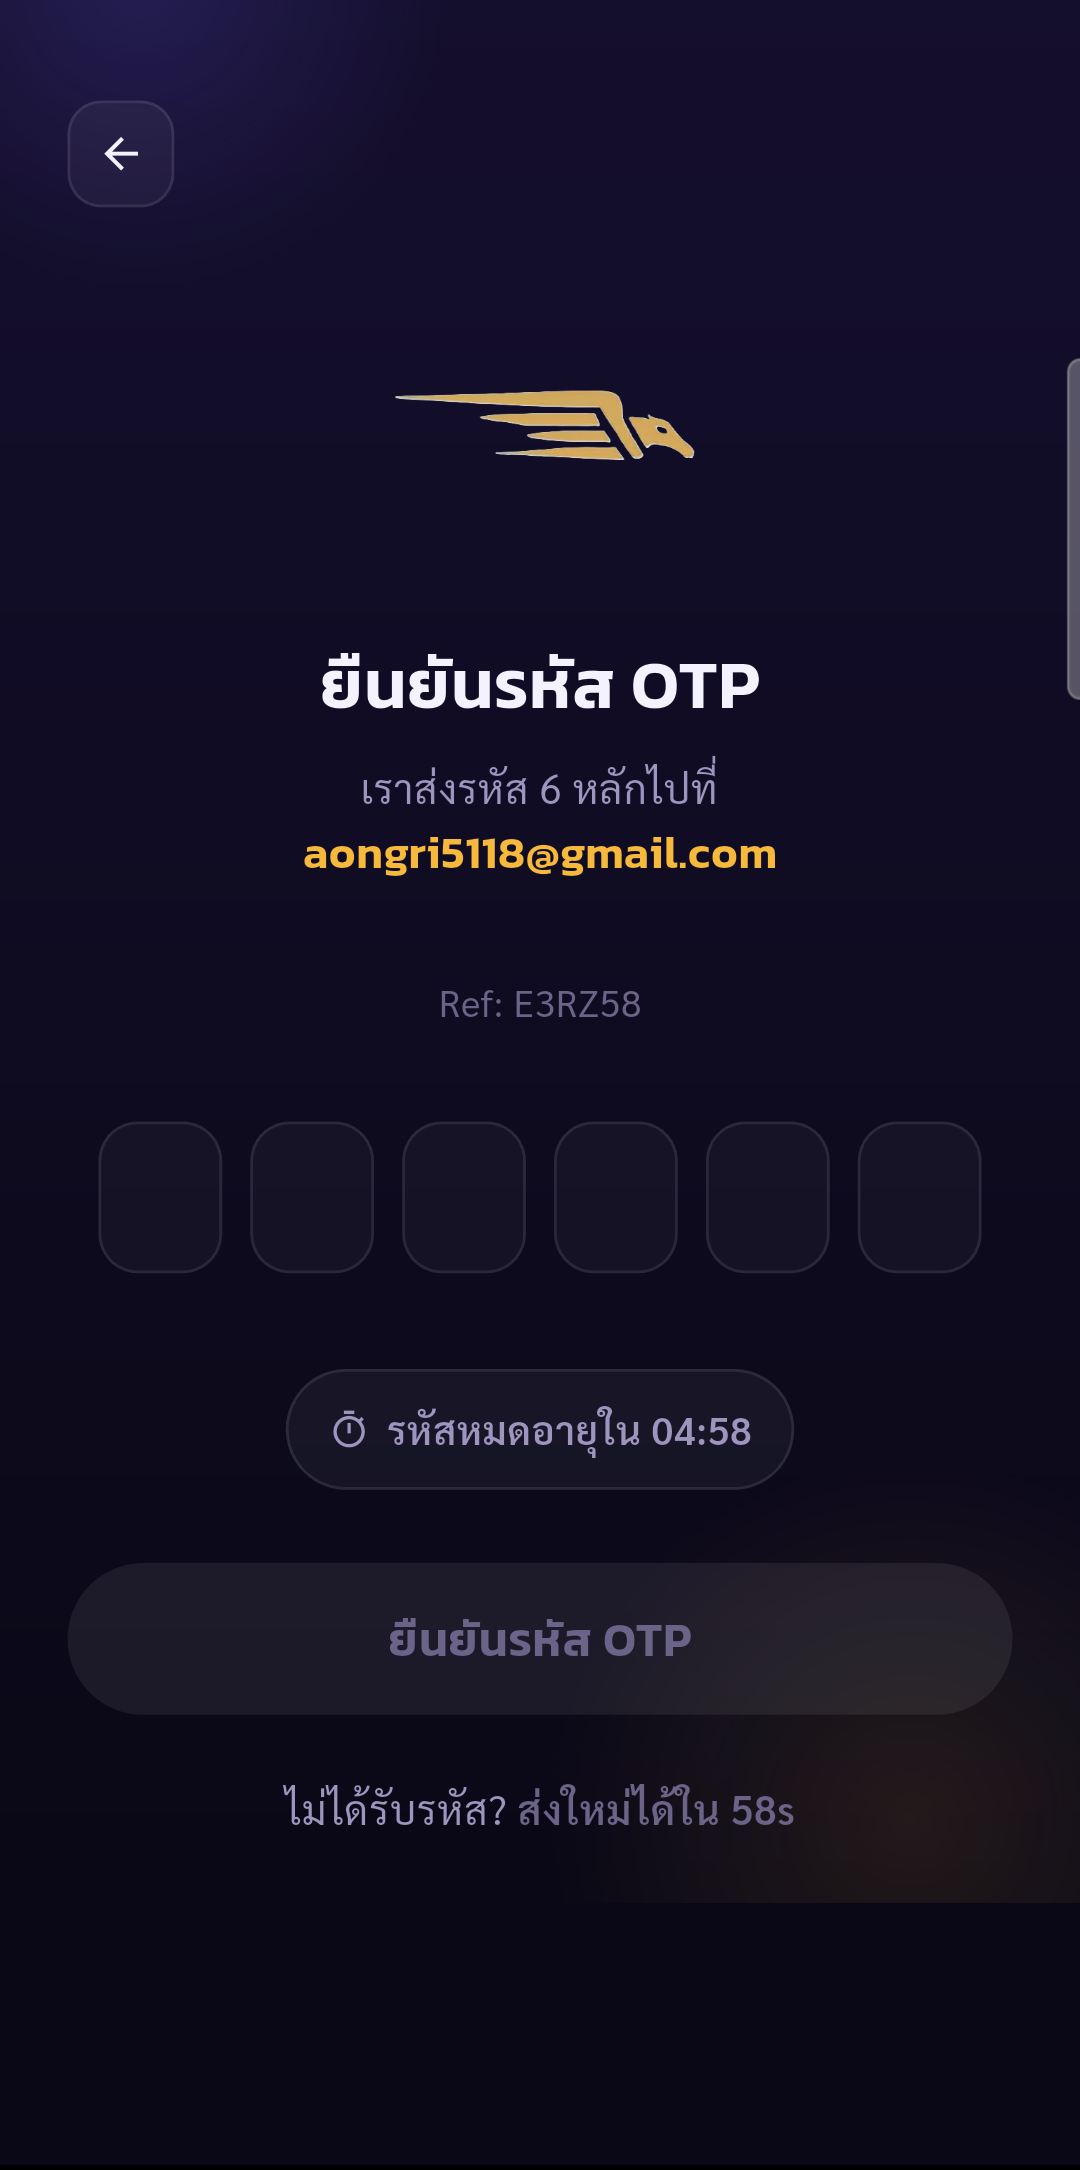
\includegraphics[width=\textwidth]{images/pegasus-otp-verification.png}\caption{ยืนยัน OTP}\end{subfigure}
\caption{หน้าจอการเข้าสู่ระบบและการสมัครสมาชิก}\label{fig:app-auth}\end{figure}

\begin{figure}[H]\centering
\begin{subfigure}[t]{0.31\textwidth}\centering
\includegraphics[width=\textwidth]{images/pegasus-terms-and-consent-unchecked.png}\caption{ยังไม่ยินยอม}\end{subfigure}\hfill
\begin{subfigure}[t]{0.31\textwidth}\centering
\includegraphics[width=\textwidth]{images/pegasus-terms-and-consent-checked.png}\caption{ยินยอมแล้ว}\end{subfigure}
\caption{หน้าข้อกำหนดและการยินยอม}\label{fig:app-consent}\end{figure}

\subsection{การเก็บข้อมูลพื้นฐานและข้อมูลสุขภาพ}

ขั้นตอน Onboarding ประกอบด้วยการกรอกวันเกิด เพศ น้ำหนัก ส่วนสูง และจำนวนวันที่ต้องการวิ่งต่อสัปดาห์ จากนั้นผู้ใช้สามารถระบุโรคประจำตัว อาการบาดเจ็บในอดีต และอาการบาดเจ็บในปัจจุบัน เพื่อให้ระบบนำไปประกอบการวางแผนการฝึก

\begin{figure}[H]\centering
\begin{subfigure}[t]{0.31\textwidth}\centering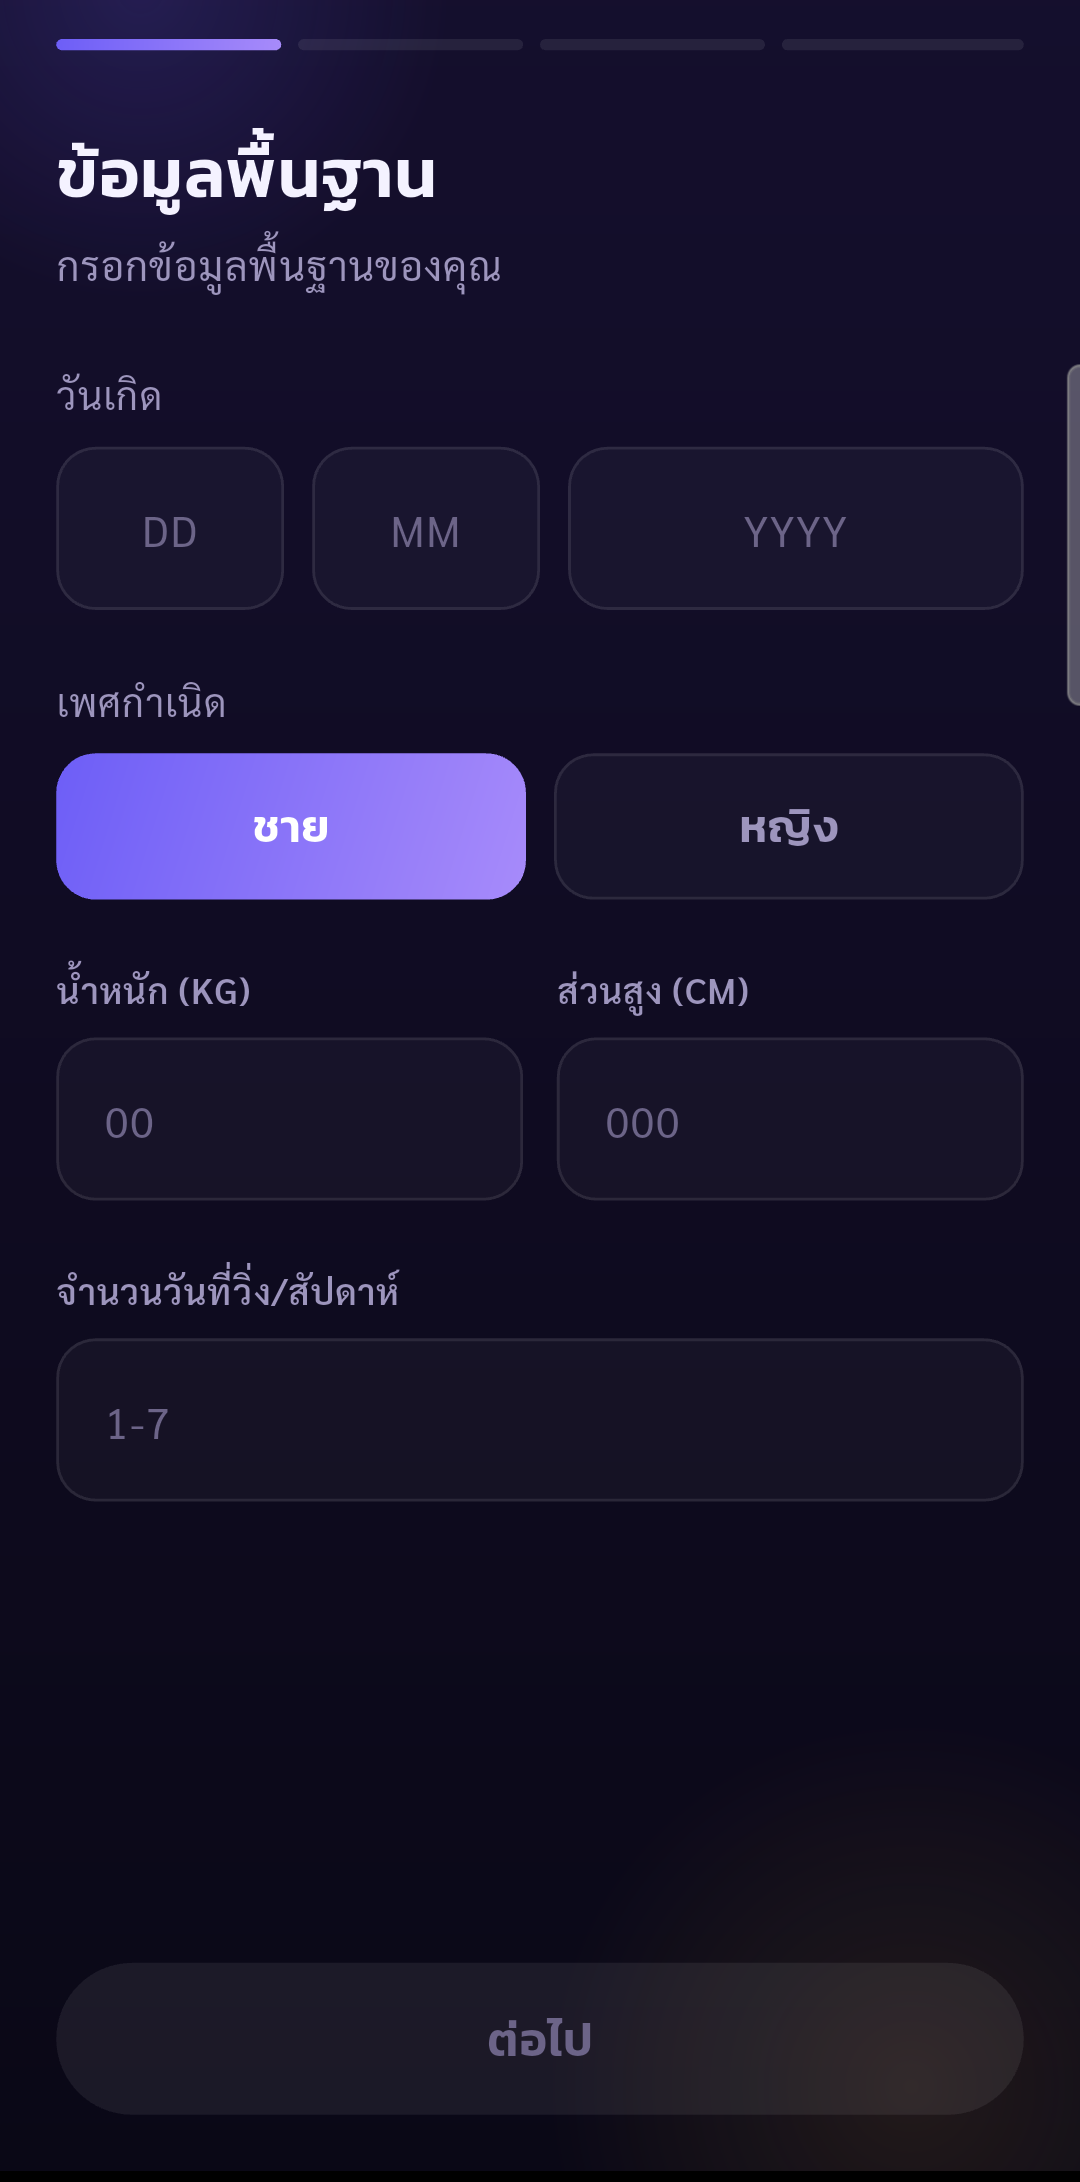
\includegraphics[width=\textwidth]{images/pegasus-onboarding-basic-information.png}\caption{ข้อมูลพื้นฐาน}\end{subfigure}\hfill
\begin{subfigure}[t]{0.31\textwidth}\centering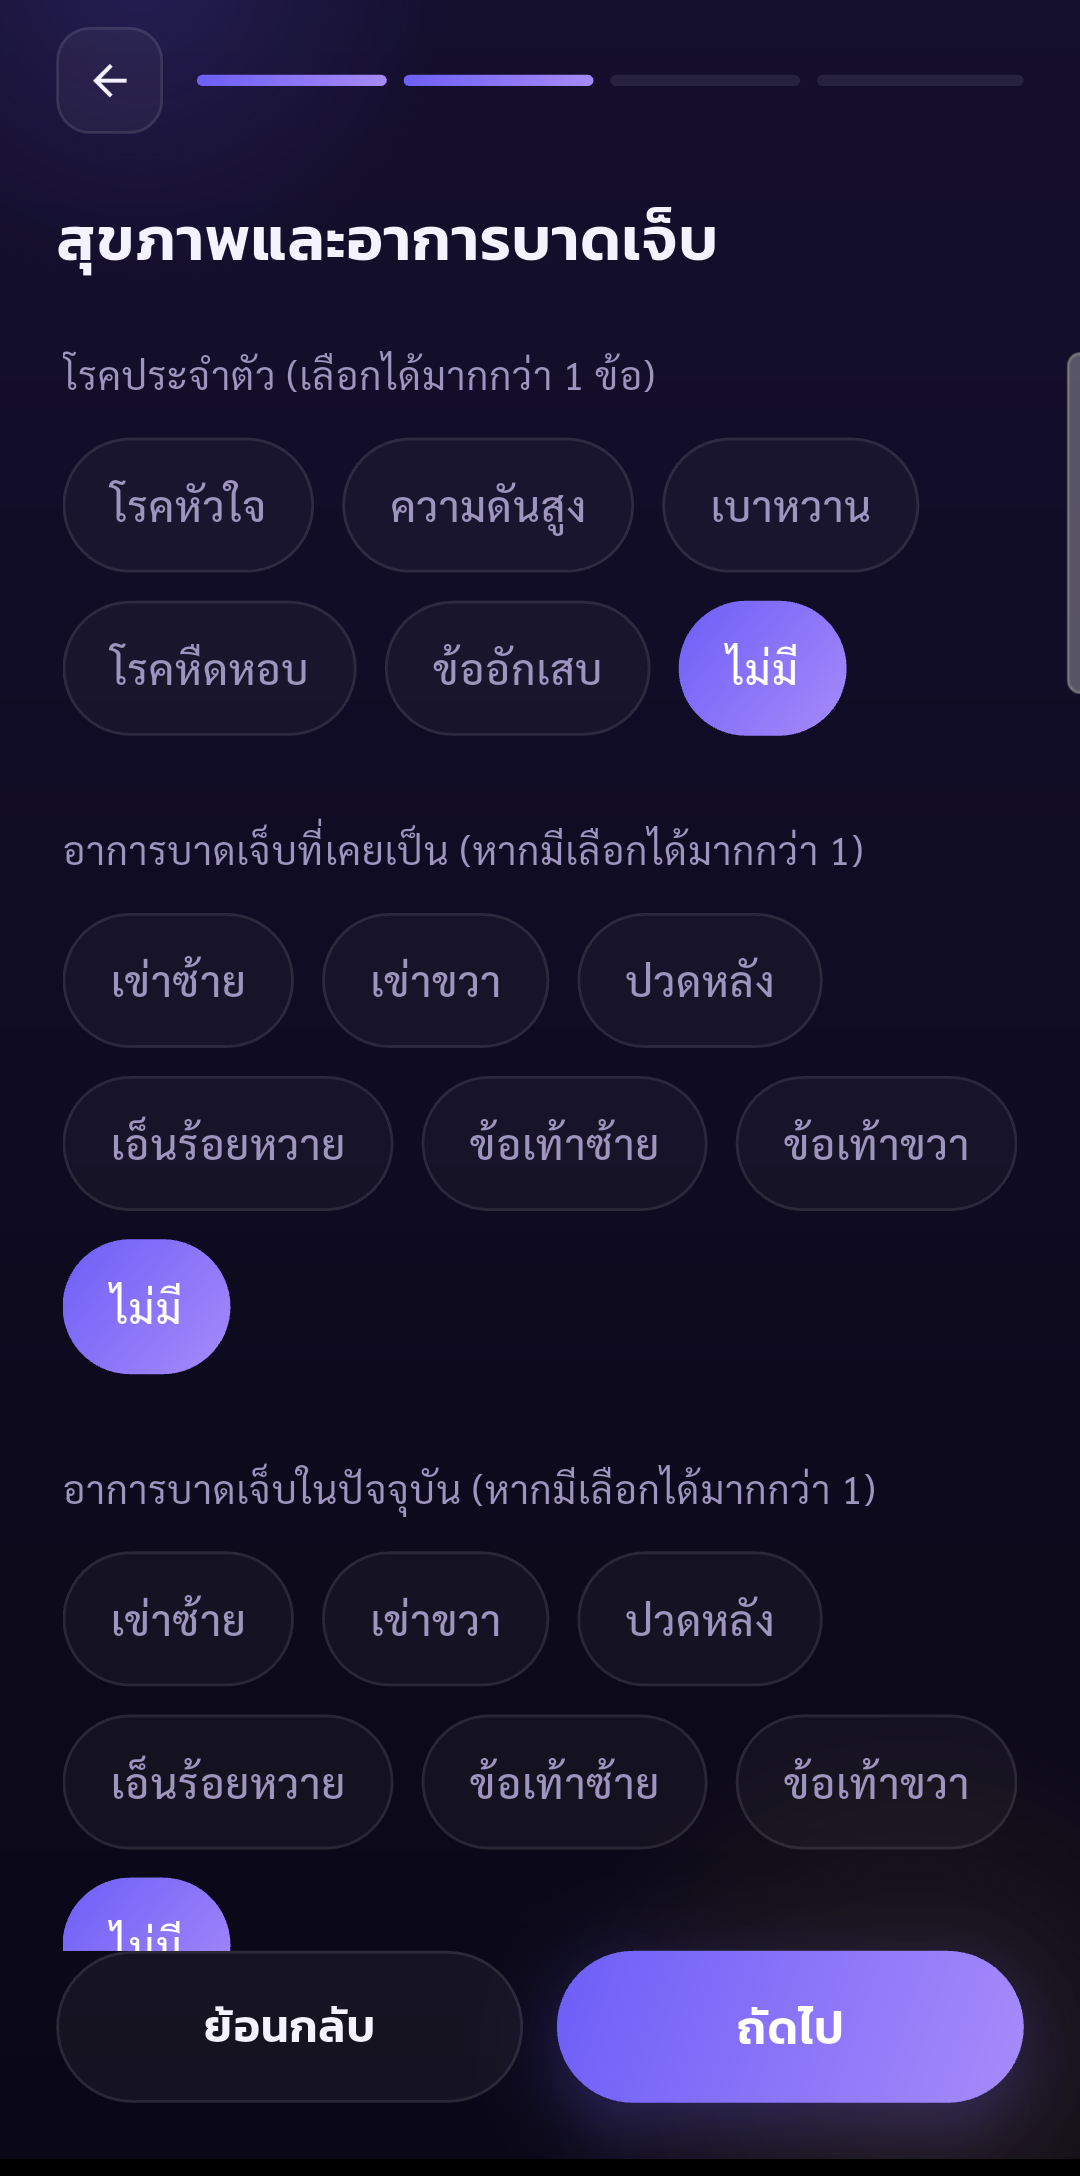
\includegraphics[width=\textwidth]{images/pegasus-onboarding-health-and-injuries.png}\caption{สุขภาพและอาการบาดเจ็บ}\end{subfigure}\hfill
\begin{subfigure}[t]{0.31\textwidth}\centering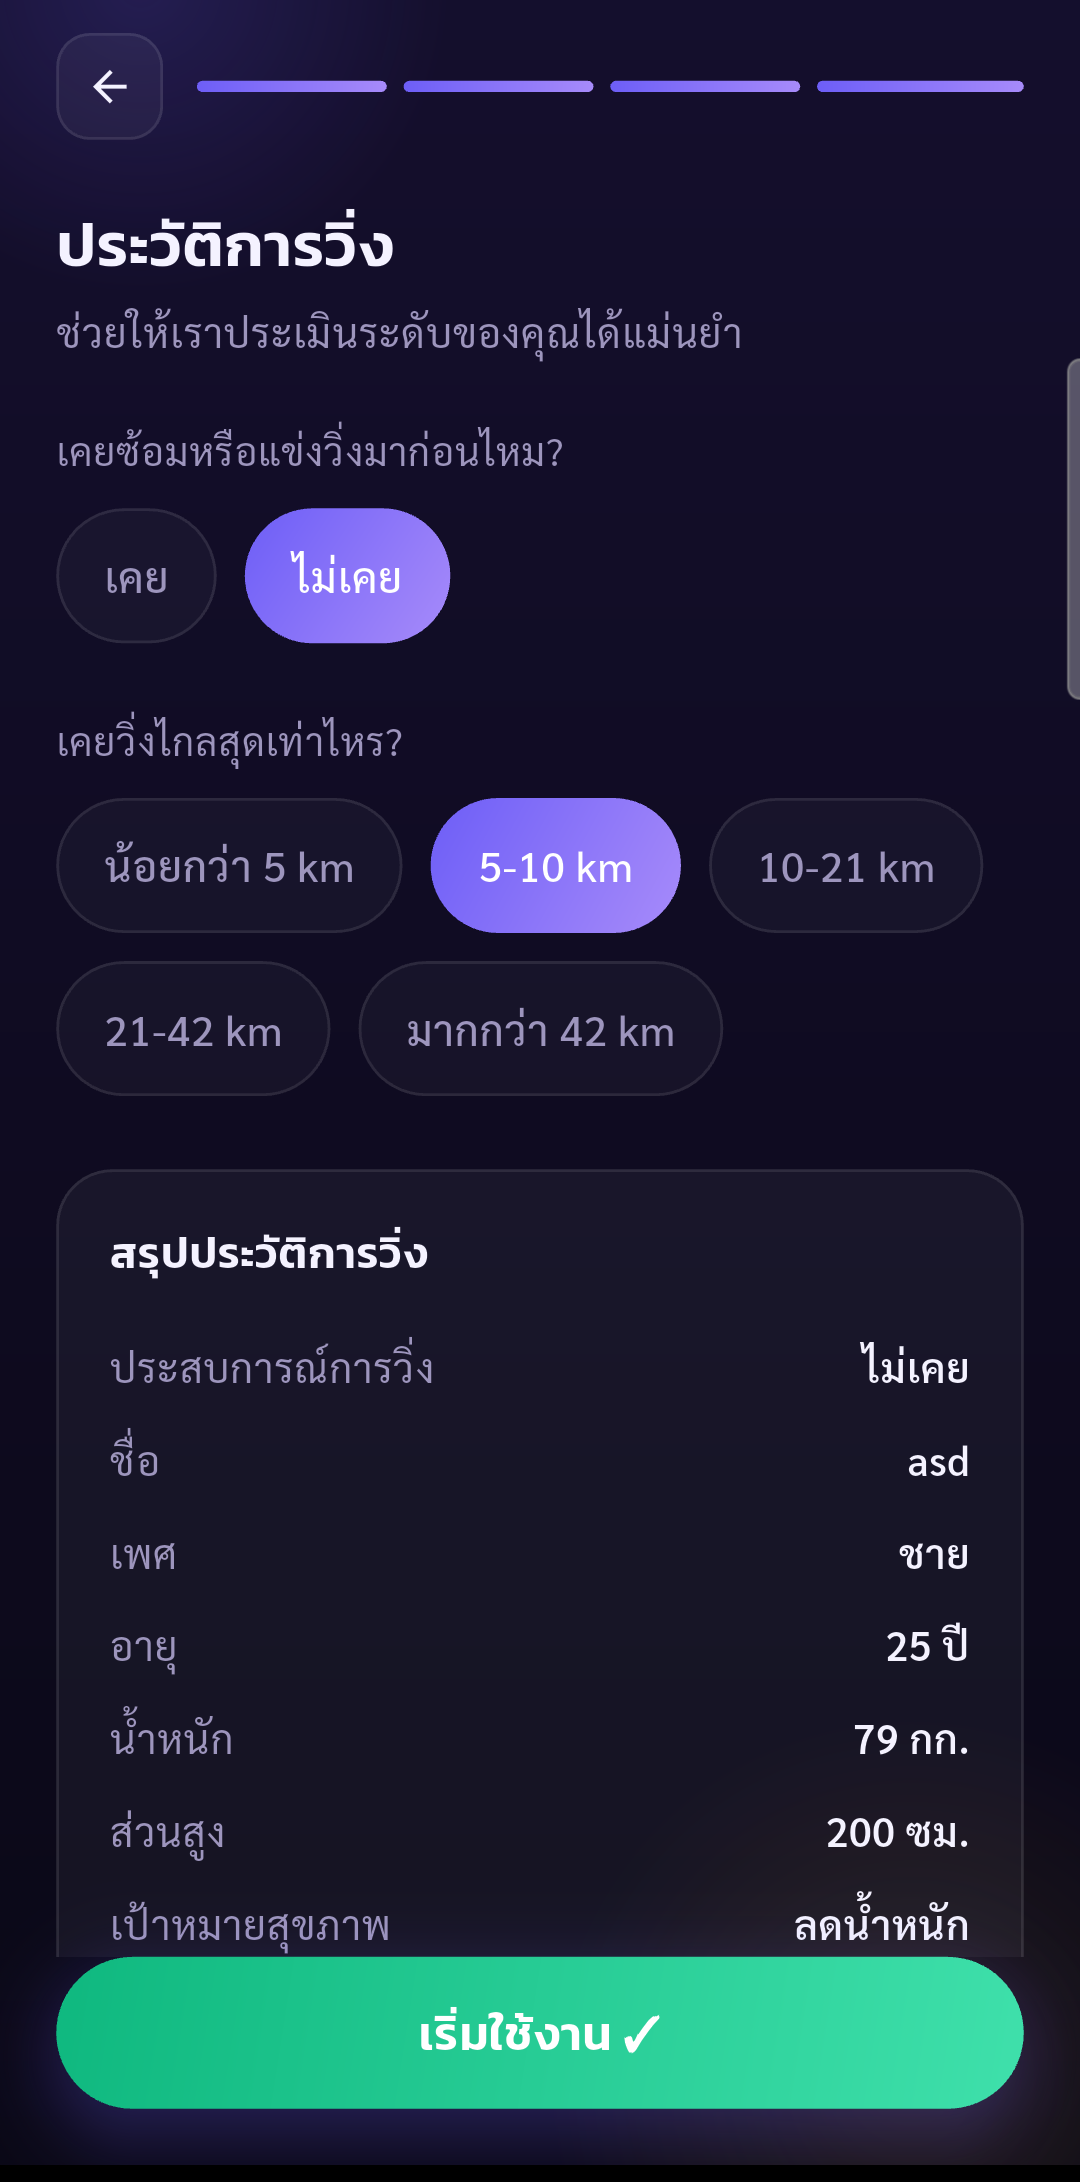
\includegraphics[width=\textwidth]{images/pegasus-onboarding-running-history-summary.png}\caption{ประวัติการวิ่ง}\end{subfigure}
\caption{หน้าจอการเก็บข้อมูลสำหรับสร้างโปรไฟล์ผู้ใช้}\label{fig:app-onboarding}\end{figure}

\subsection{การกำหนดเป้าหมายการวิ่ง}

ผู้ใช้สามารถเลือกเป้าหมายด้านระยะทาง เช่น 5K, 10K, Half Marathon หรือ Full Marathon และเลือกเป้าหมายด้านสุขภาพ เช่น ลดน้ำหนัก เพิ่มกล้ามเนื้อ เพิ่มความเร็ว เพิ่มความอึด หรือสร้างวินัย ระบบจะใช้ข้อมูลดังกล่าวเป็นเงื่อนไขเริ่มต้นของ Adaptive Training Engine

\begin{figure}[H]\centering
\begin{subfigure}[t]{0.31\textwidth}\centering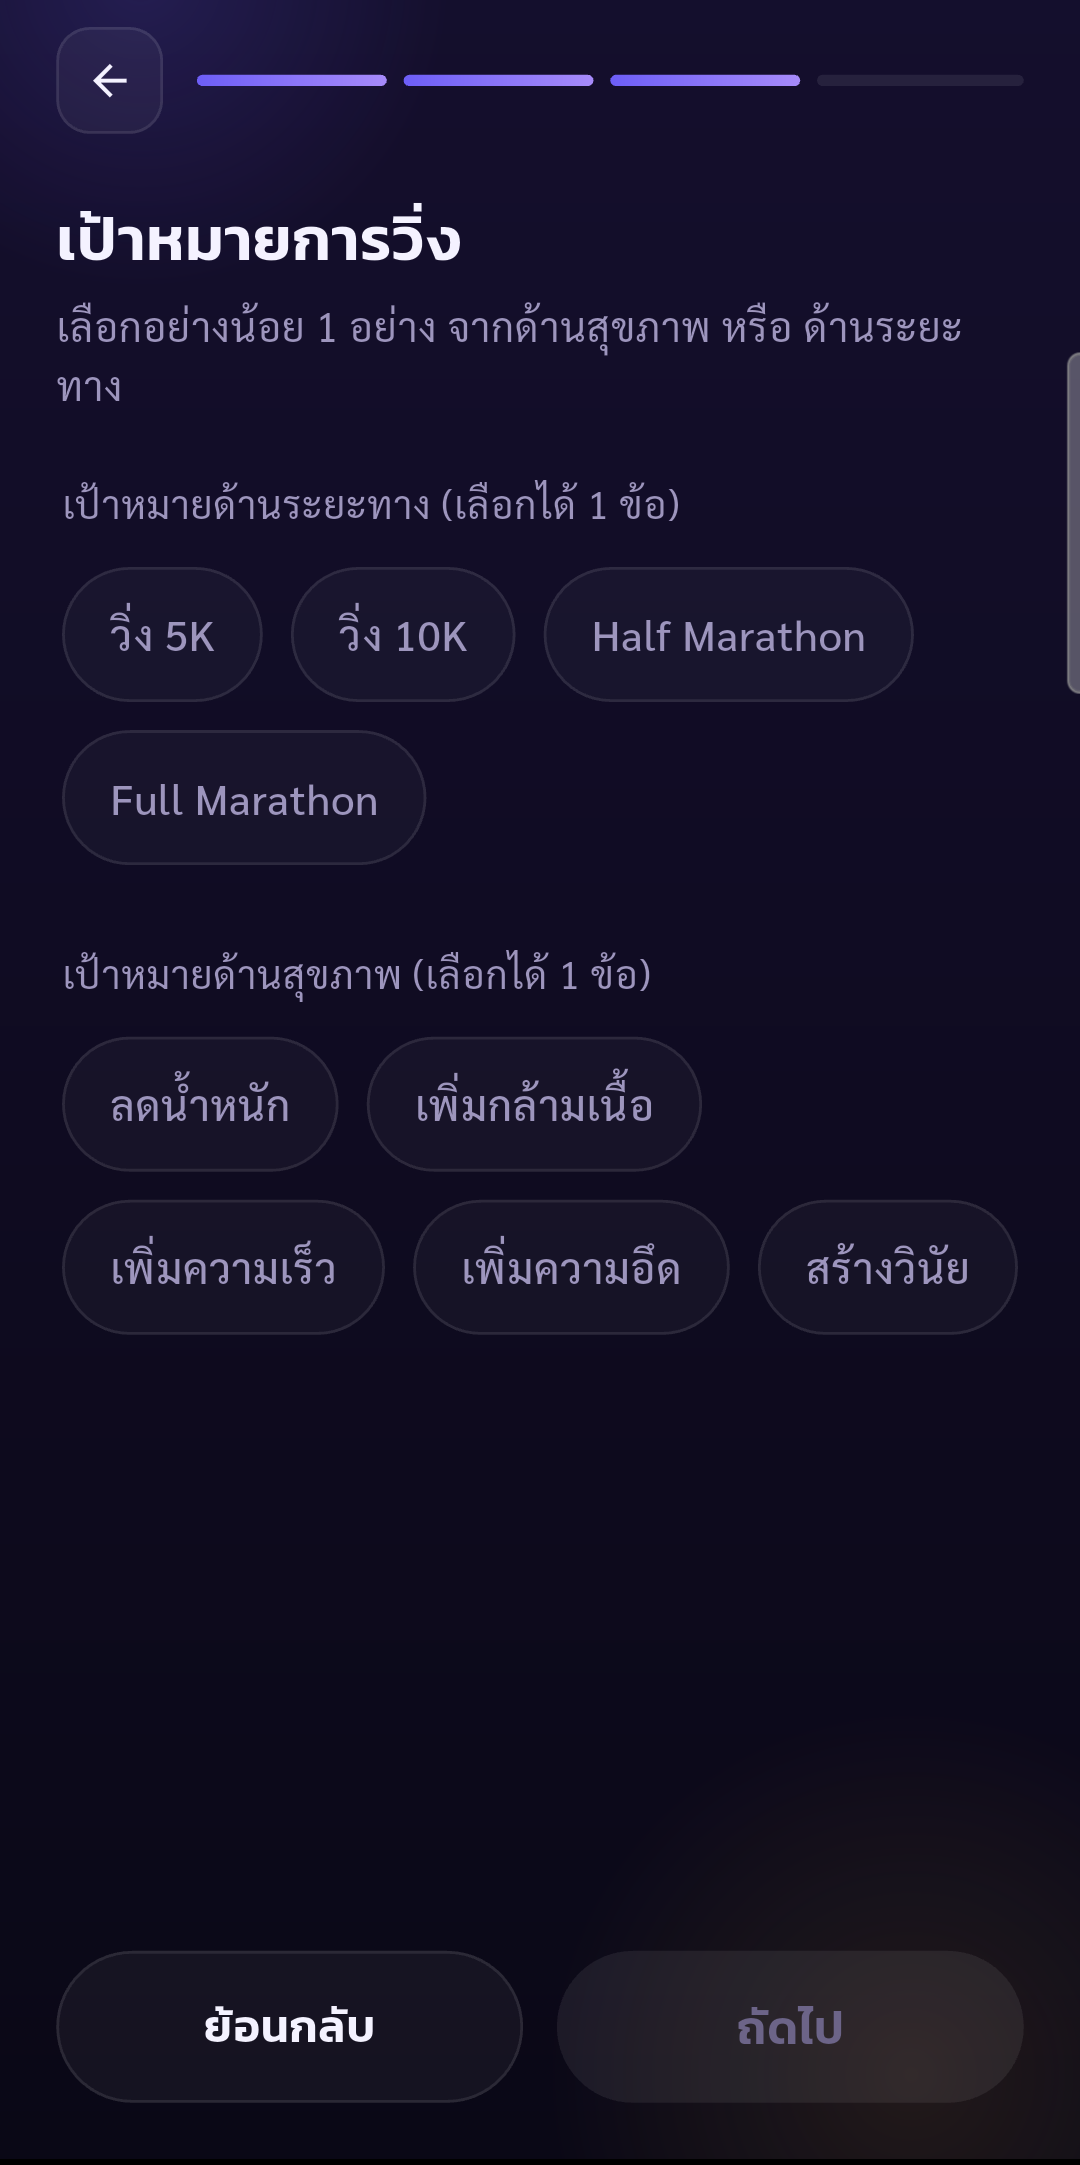
\includegraphics[width=\textwidth]{images/pegasus-onboarding-running-goals.png}\caption{เป้าหมายการวิ่ง}\end{subfigure}\hfill
\begin{subfigure}[t]{0.31\textwidth}\centering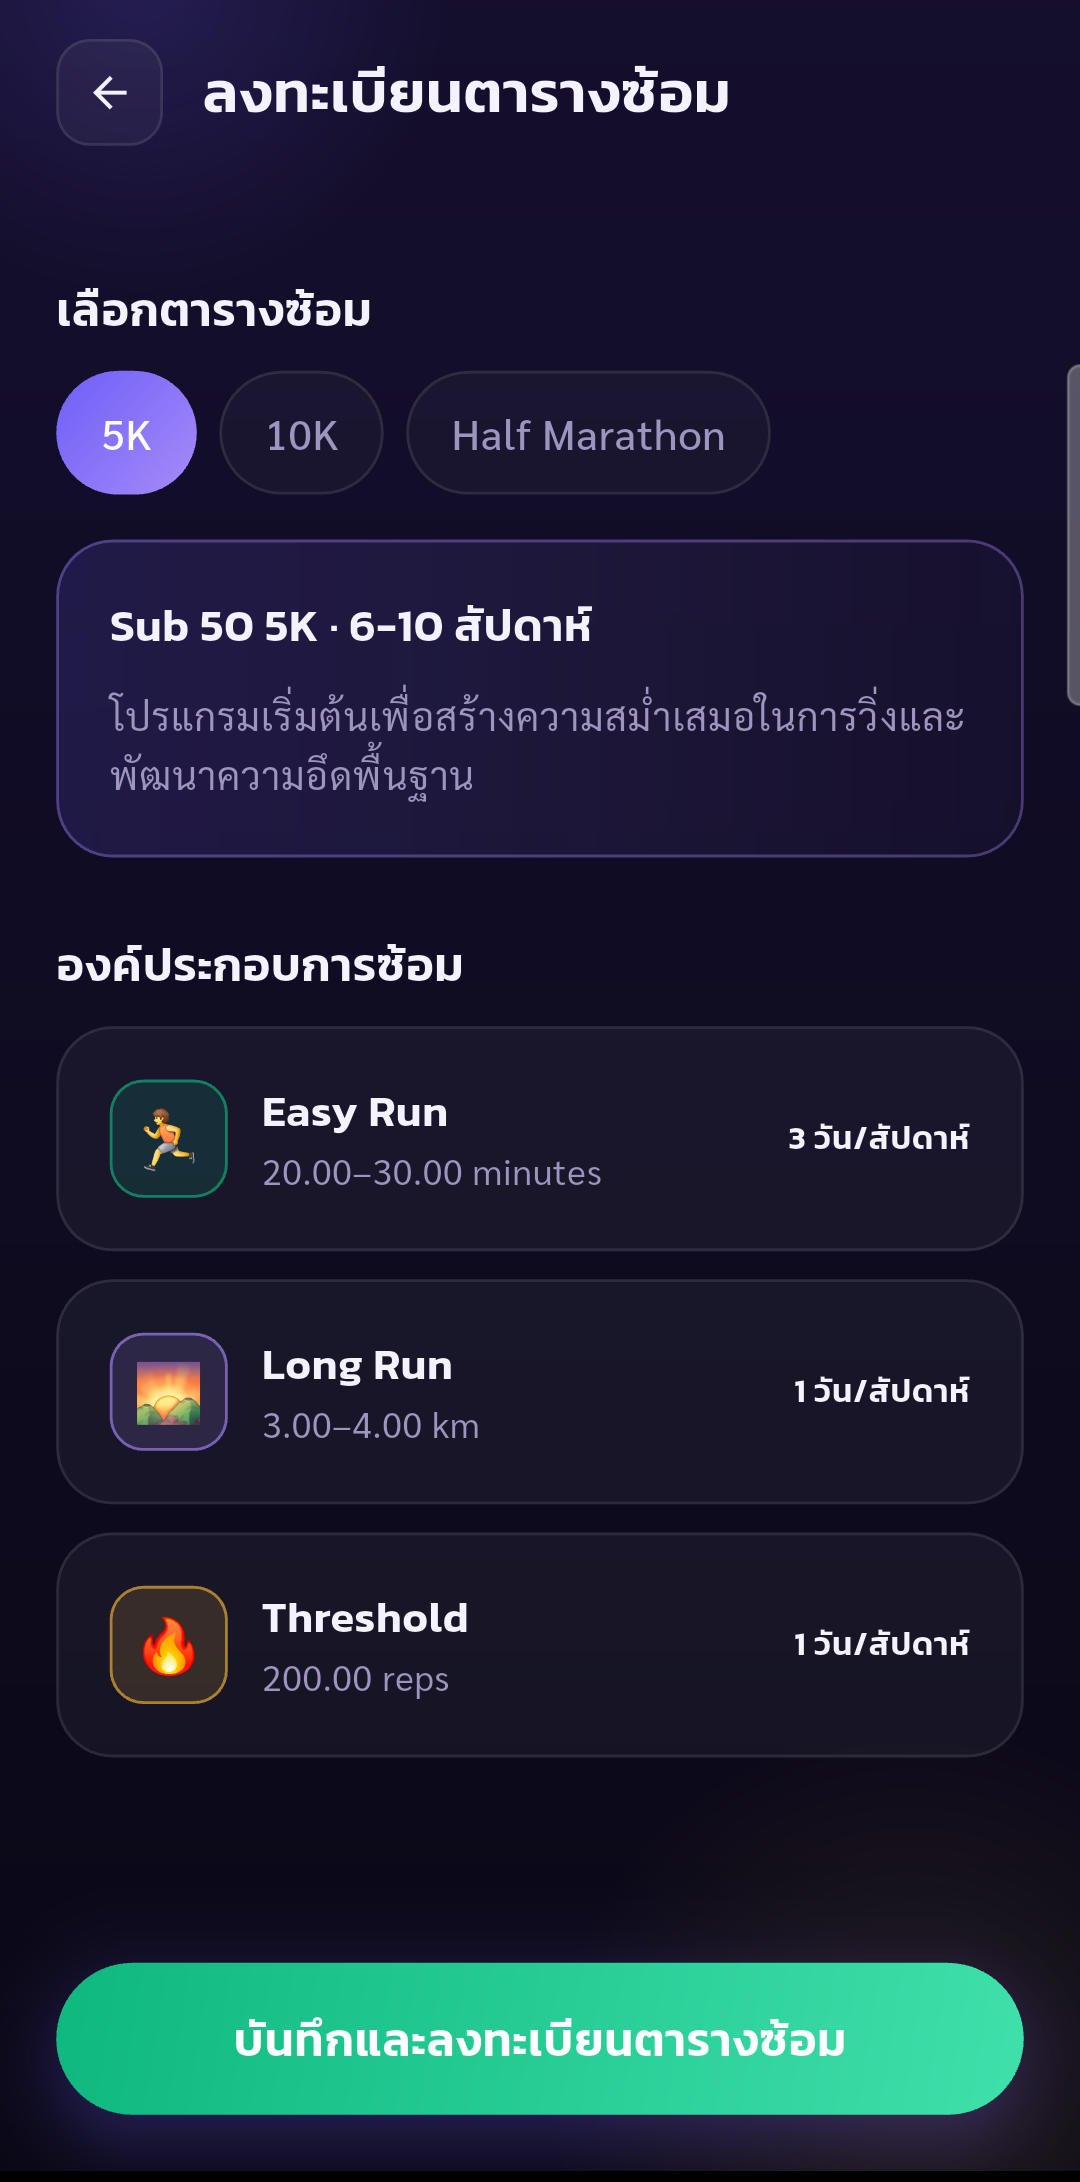
\includegraphics[width=\textwidth]{images/pegasus-training-plan-5k.png}\caption{แผน 5K}\end{subfigure}\hfill
\begin{subfigure}[t]{0.31\textwidth}\centering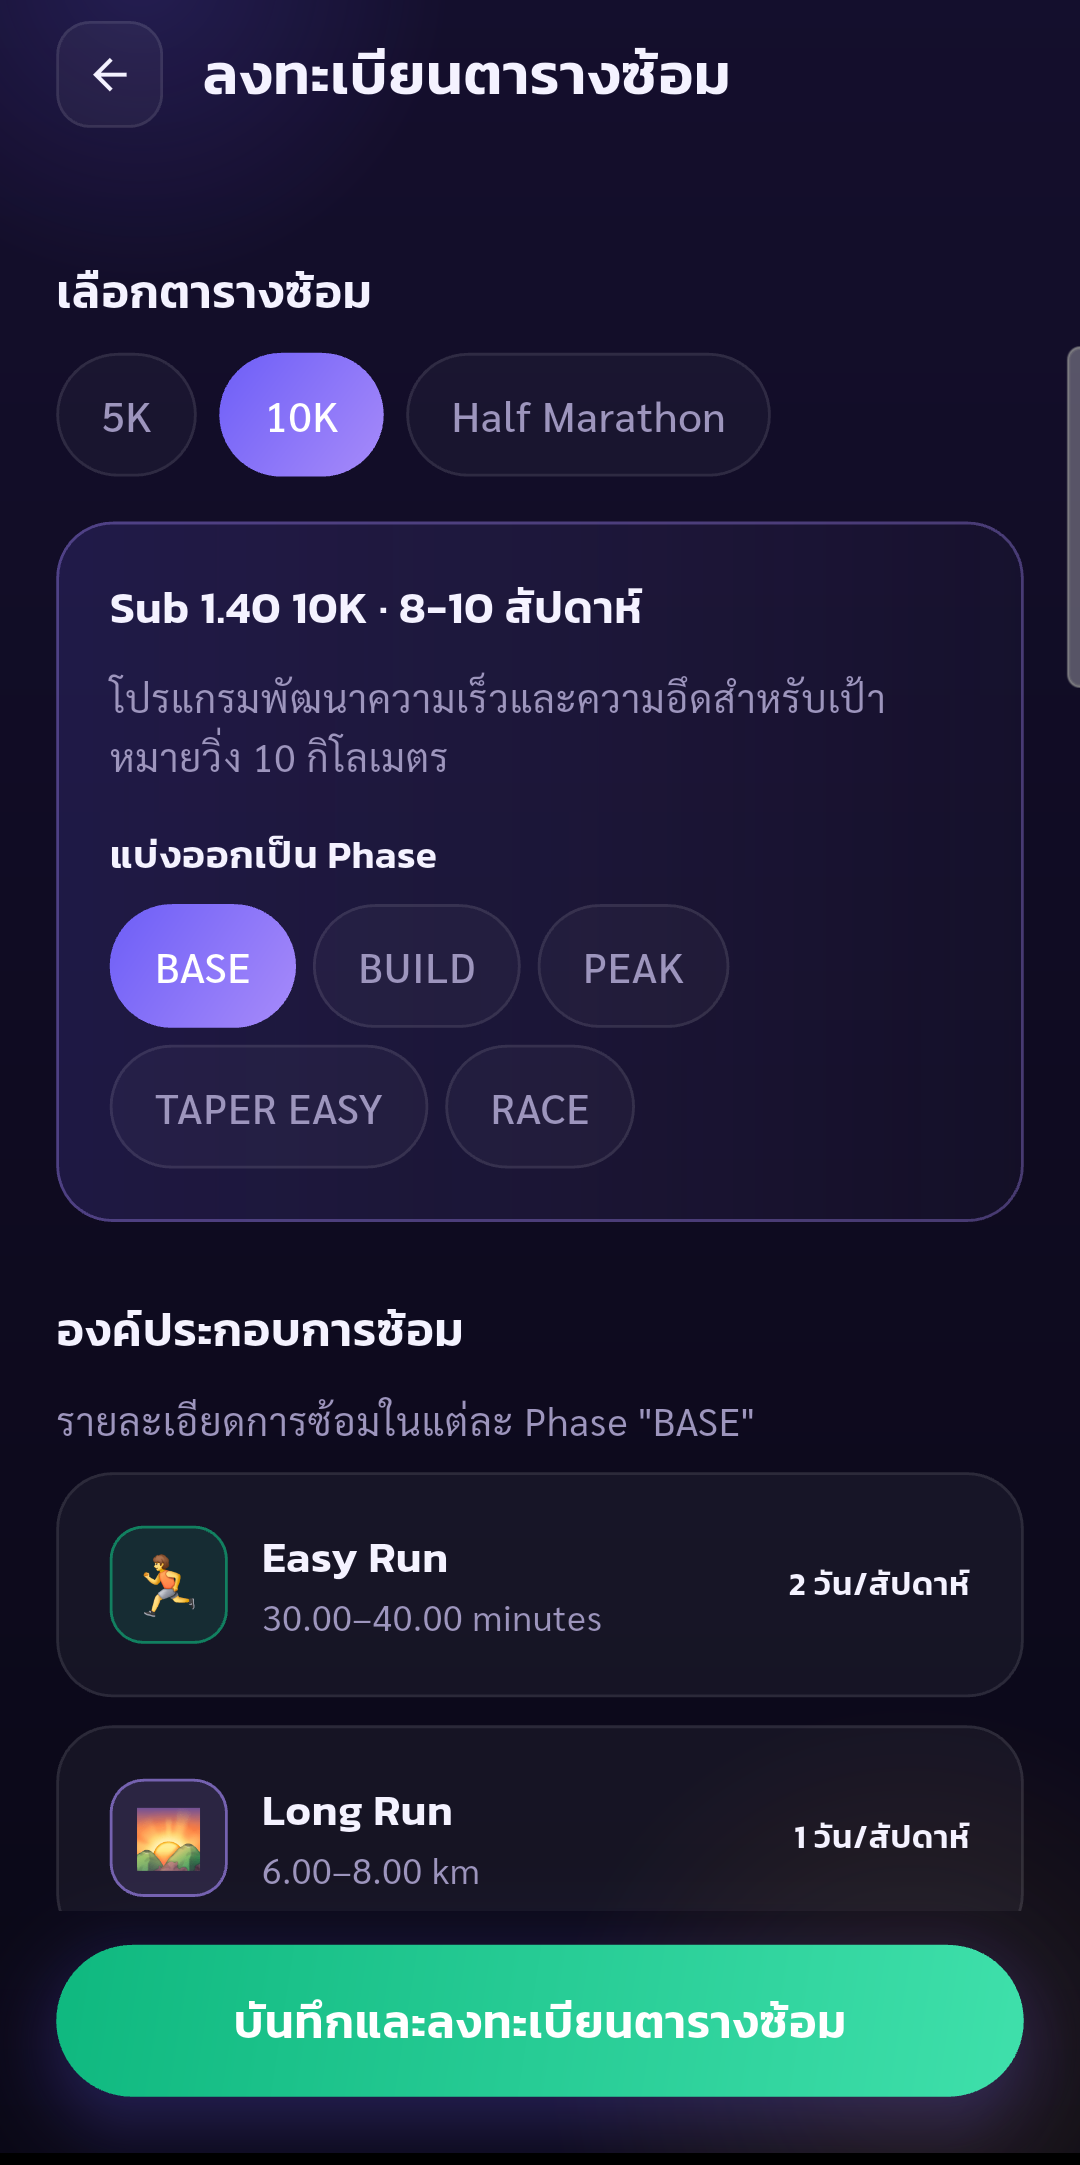
\includegraphics[width=\textwidth]{images/pegasus-training-plan-10k.png}\caption{แผน 10K}\end{subfigure}
\caption{การกำหนดเป้าหมายและการเลือกแผนการฝึก}\label{fig:app-goals}\end{figure}

\begin{figure}[H]\centering
\begin{subfigure}[t]{0.31\textwidth}\centering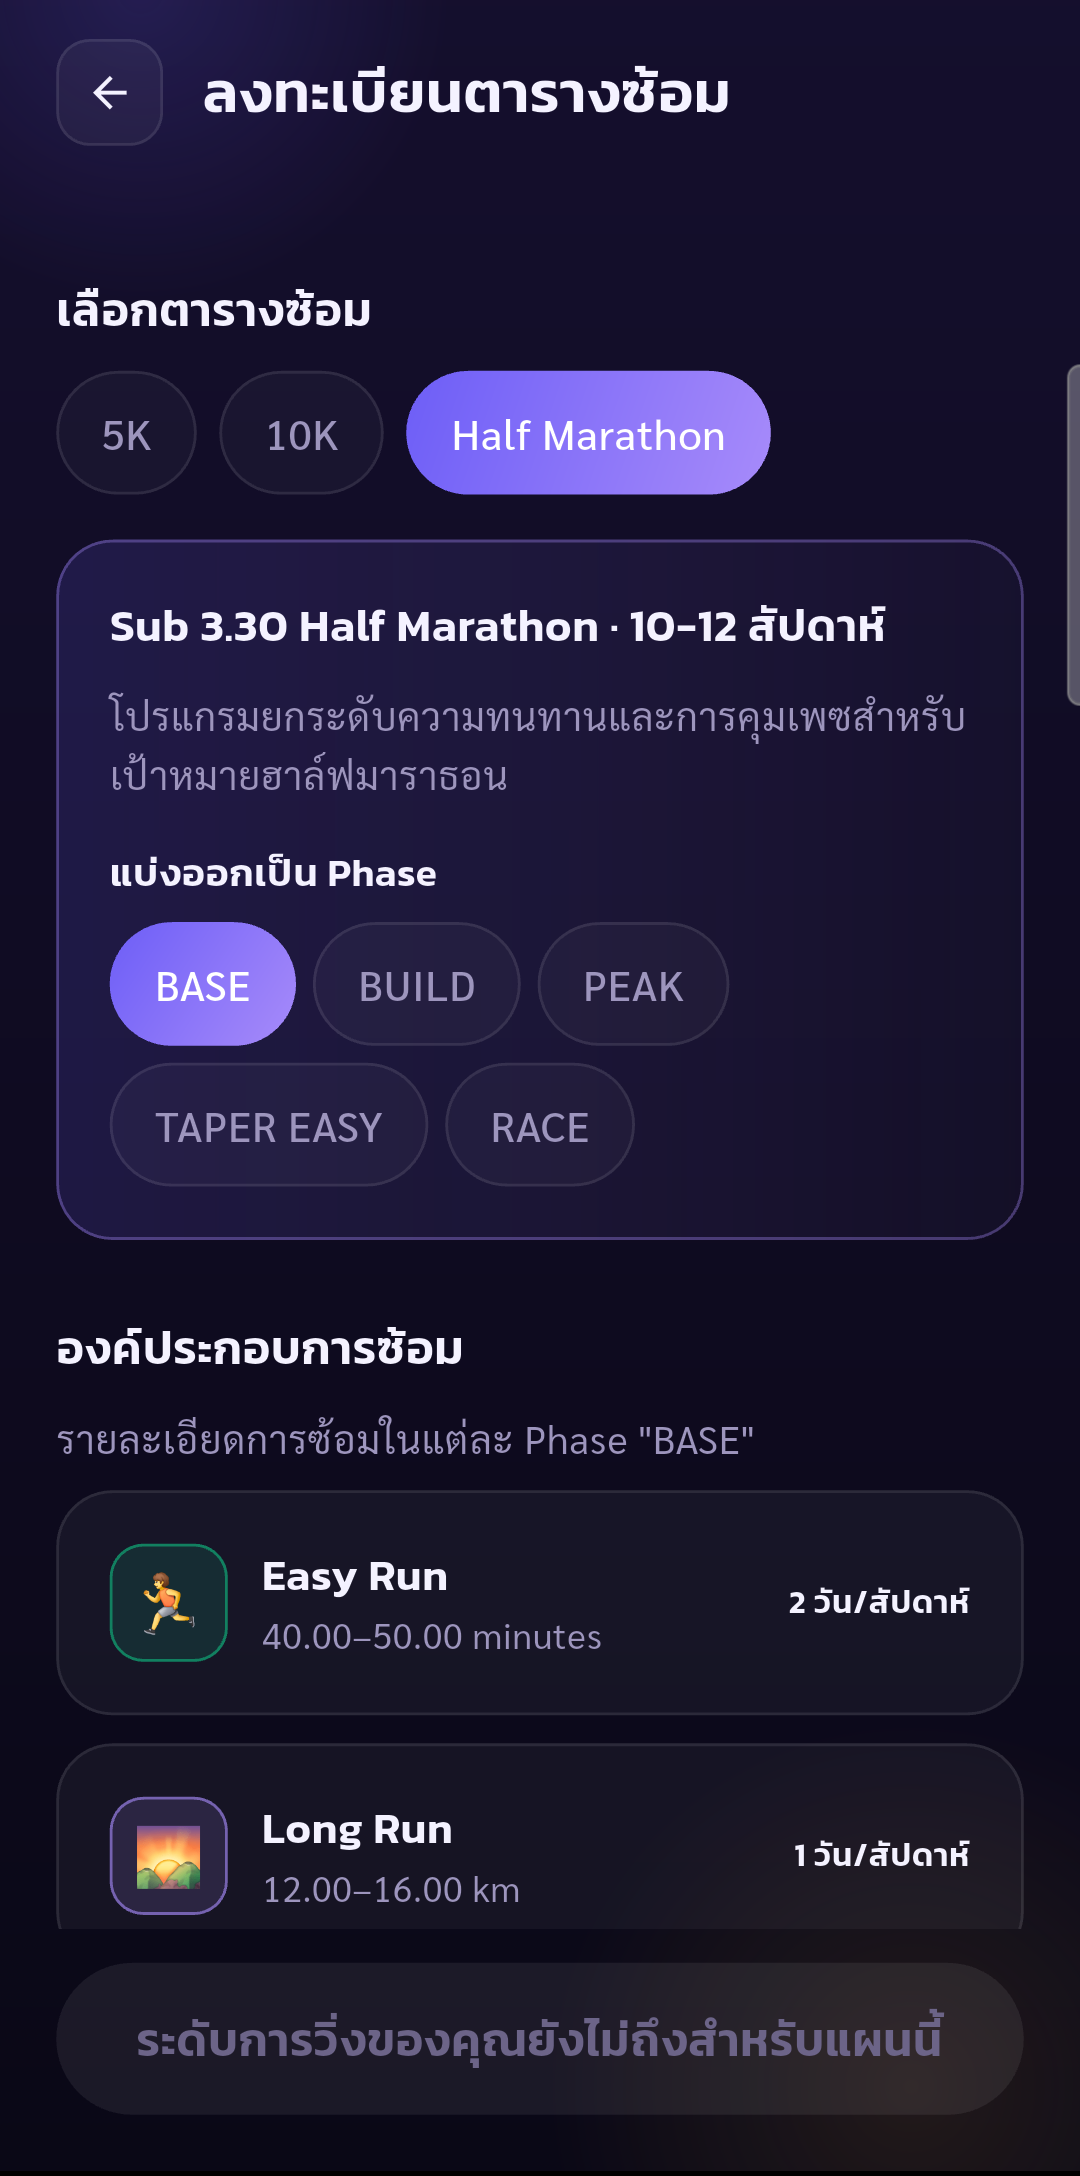
\includegraphics[width=\textwidth]{images/pegasus-training-plan-half-marathon.png}\caption{แผน Half Marathon}\end{subfigure}\hfill
\begin{subfigure}[t]{0.31\textwidth}\centering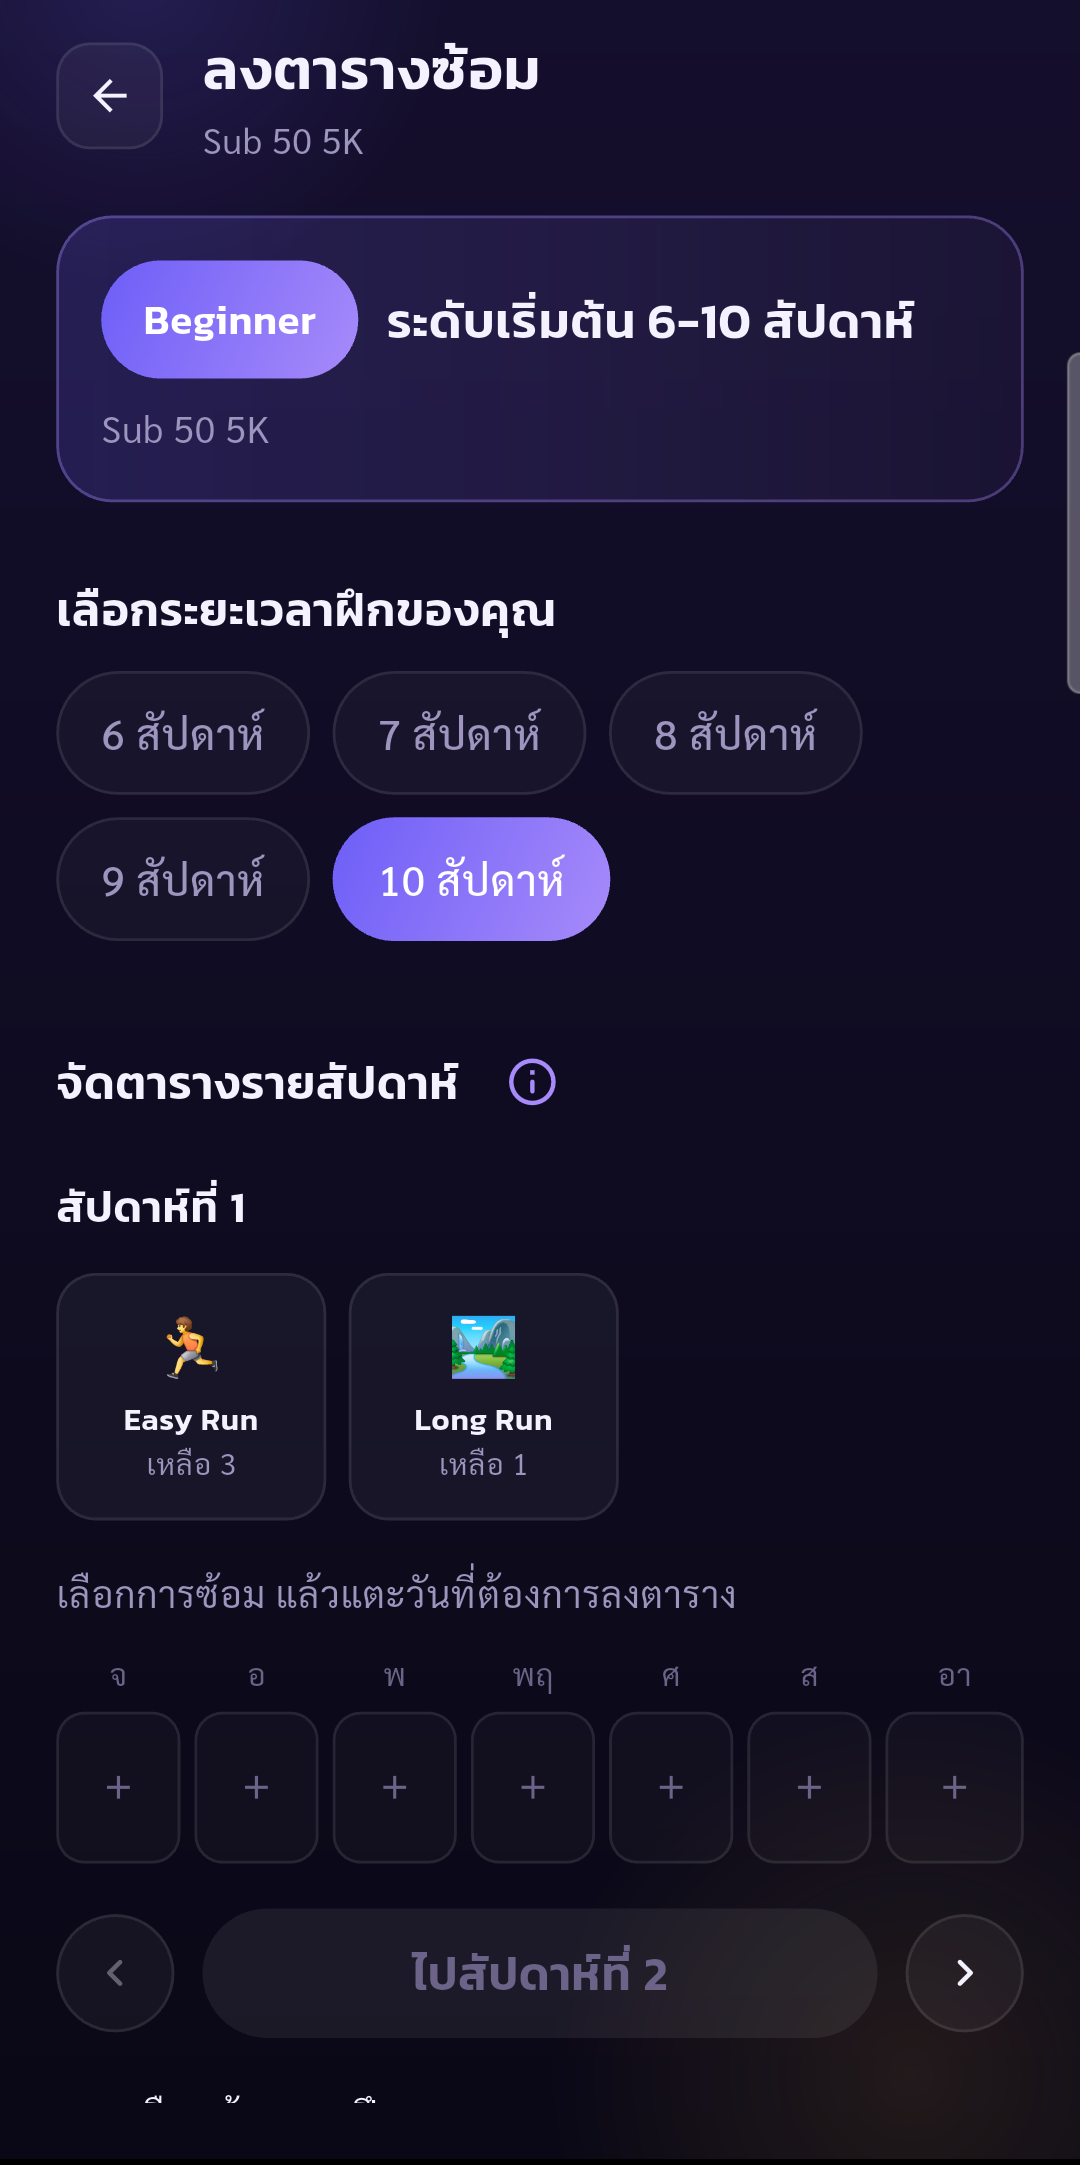
\includegraphics[width=\textwidth]{images/pegasus-schedule-builder-5k.png}\caption{จัดตารางแผน 5K}\end{subfigure}\hfill
\begin{subfigure}[t]{0.31\textwidth}\centering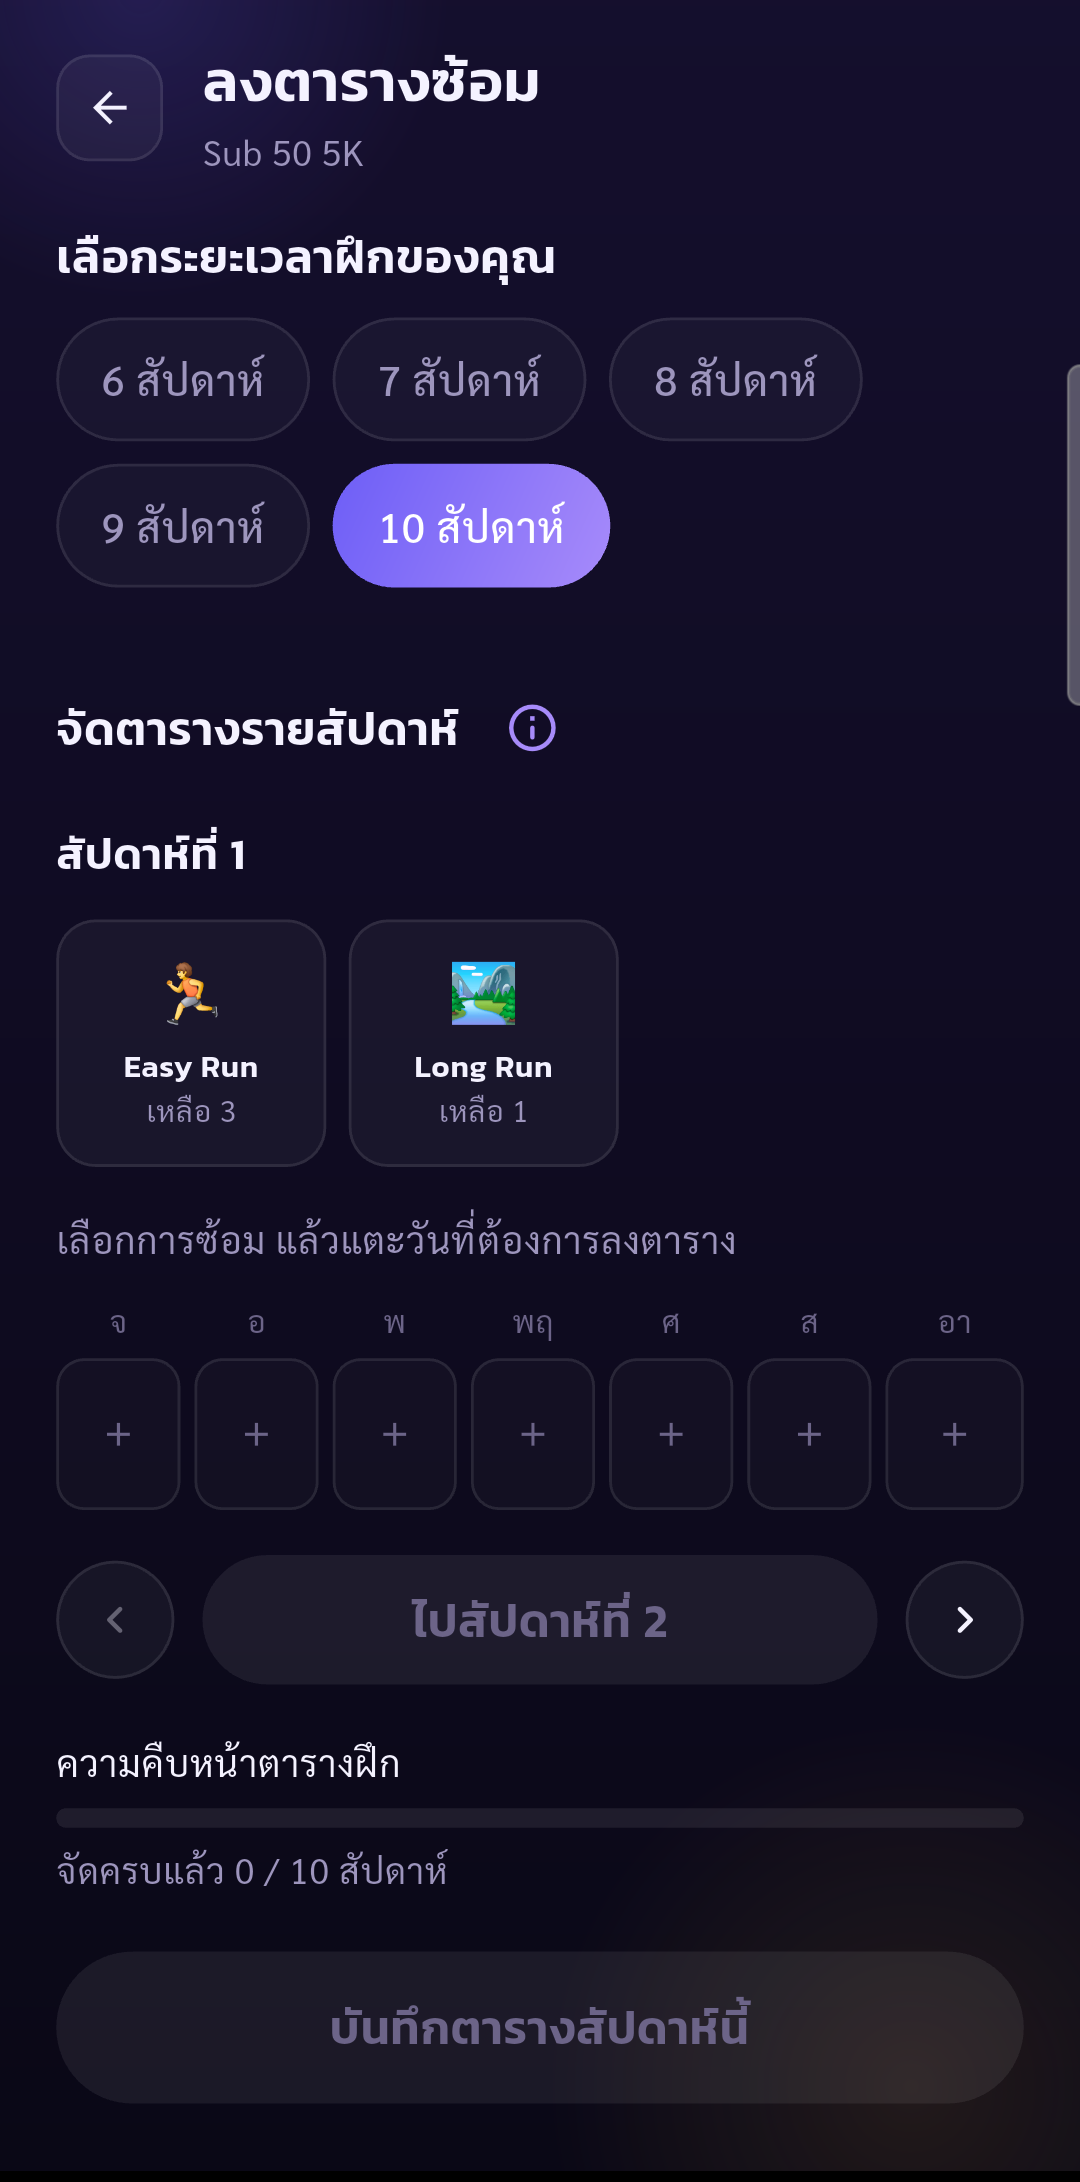
\includegraphics[width=\textwidth]{images/pegasus-schedule-builder-progress.png}\caption{ความคืบหน้าตารางฝึก}\end{subfigure}
\caption{รายละเอียดแผนการฝึกและการจัดตารางรายสัปดาห์}\label{fig:app-plans}\end{figure}

\subsection{หน้าหลักและ Daily Wellness Check-in}

หน้าหลักแสดงข้อมูลผู้ใช้ คะแนน เหรียญ กิจกรรมที่ต้องทำ Session การวิ่ง และแผนการฝึก ส่วน Daily Wellness Check-in ใช้ให้ผู้ใช้ประเมินคุณภาพการนอน จำนวนชั่วโมงนอน ความเมื่อยล้ากล้ามเนื้อ ระดับพลังกล้ามเนื้อ และระดับความเครียด เพื่อนำไปปรับความเหมาะสมของการฝึกในวันนั้น

\begin{figure}[H]\centering
\begin{subfigure}[t]{0.31\textwidth}\centering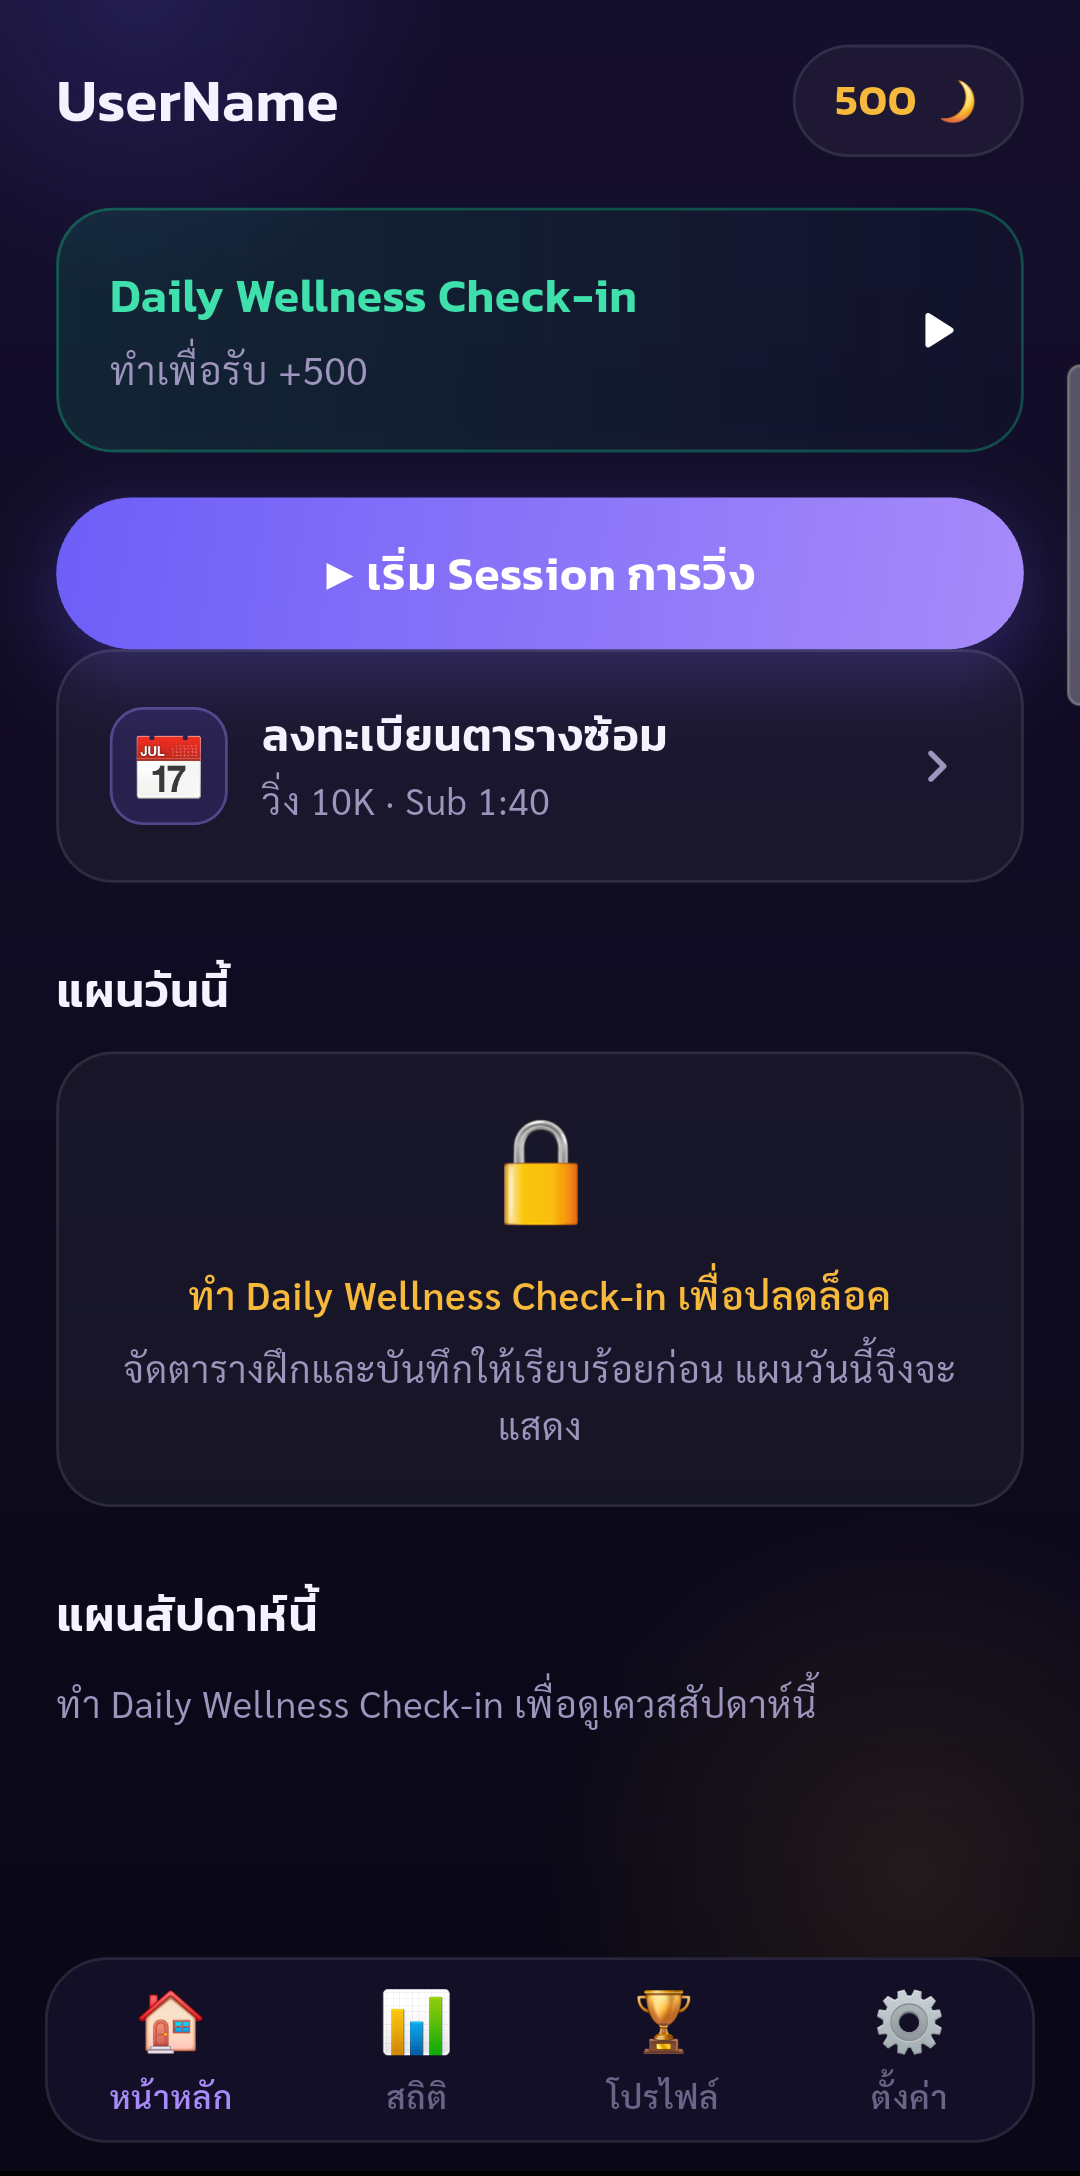
\includegraphics[width=\textwidth]{images/pegasus-home-locked.png}\caption{หน้าหลักก่อนปลดล็อก}\end{subfigure}\hfill
\begin{subfigure}[t]{0.31\textwidth}\centering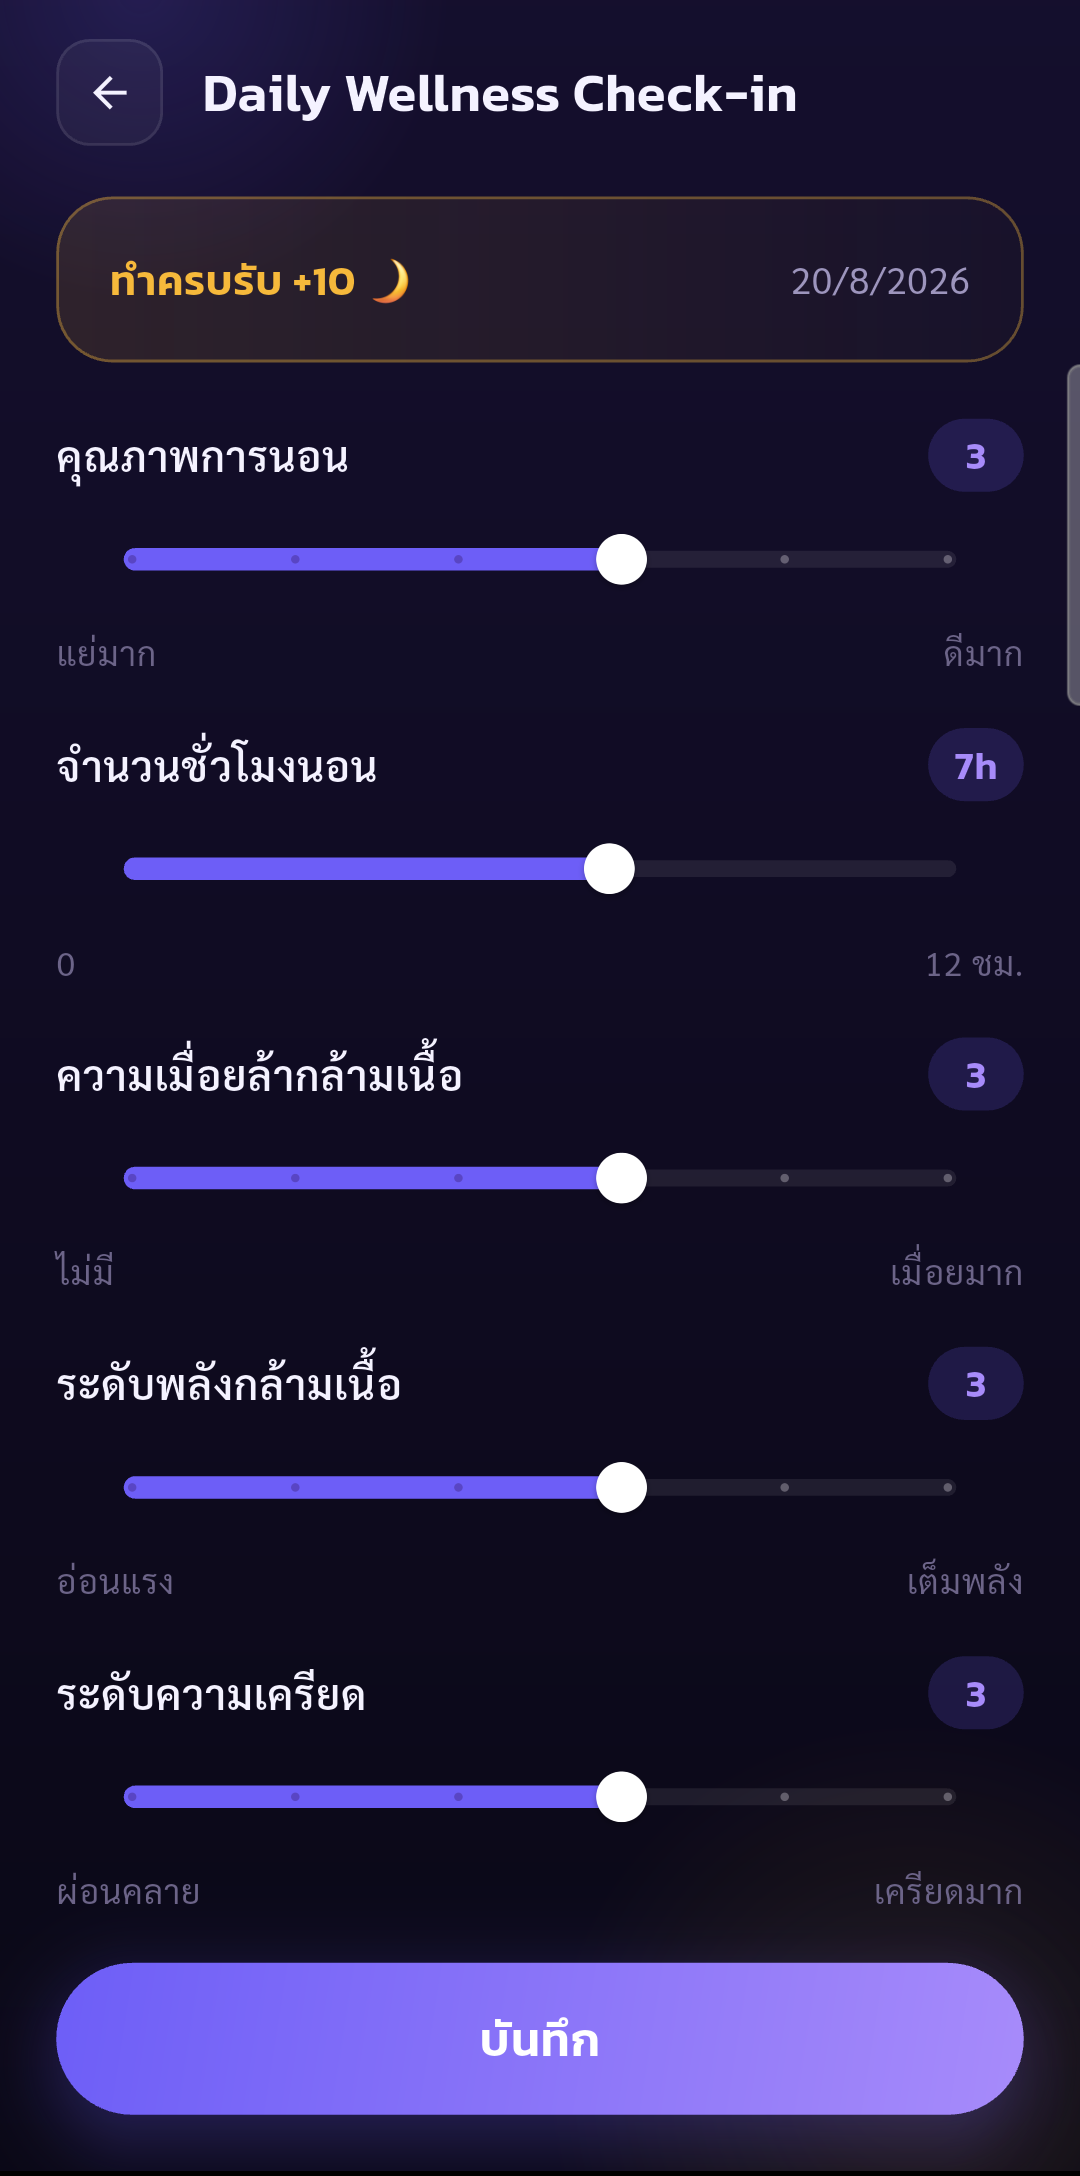
\includegraphics[width=\textwidth]{images/pegasus-daily-wellness-check-in.png}\caption{Daily Wellness Check-in}\end{subfigure}\hfill
\begin{subfigure}[t]{0.31\textwidth}\centering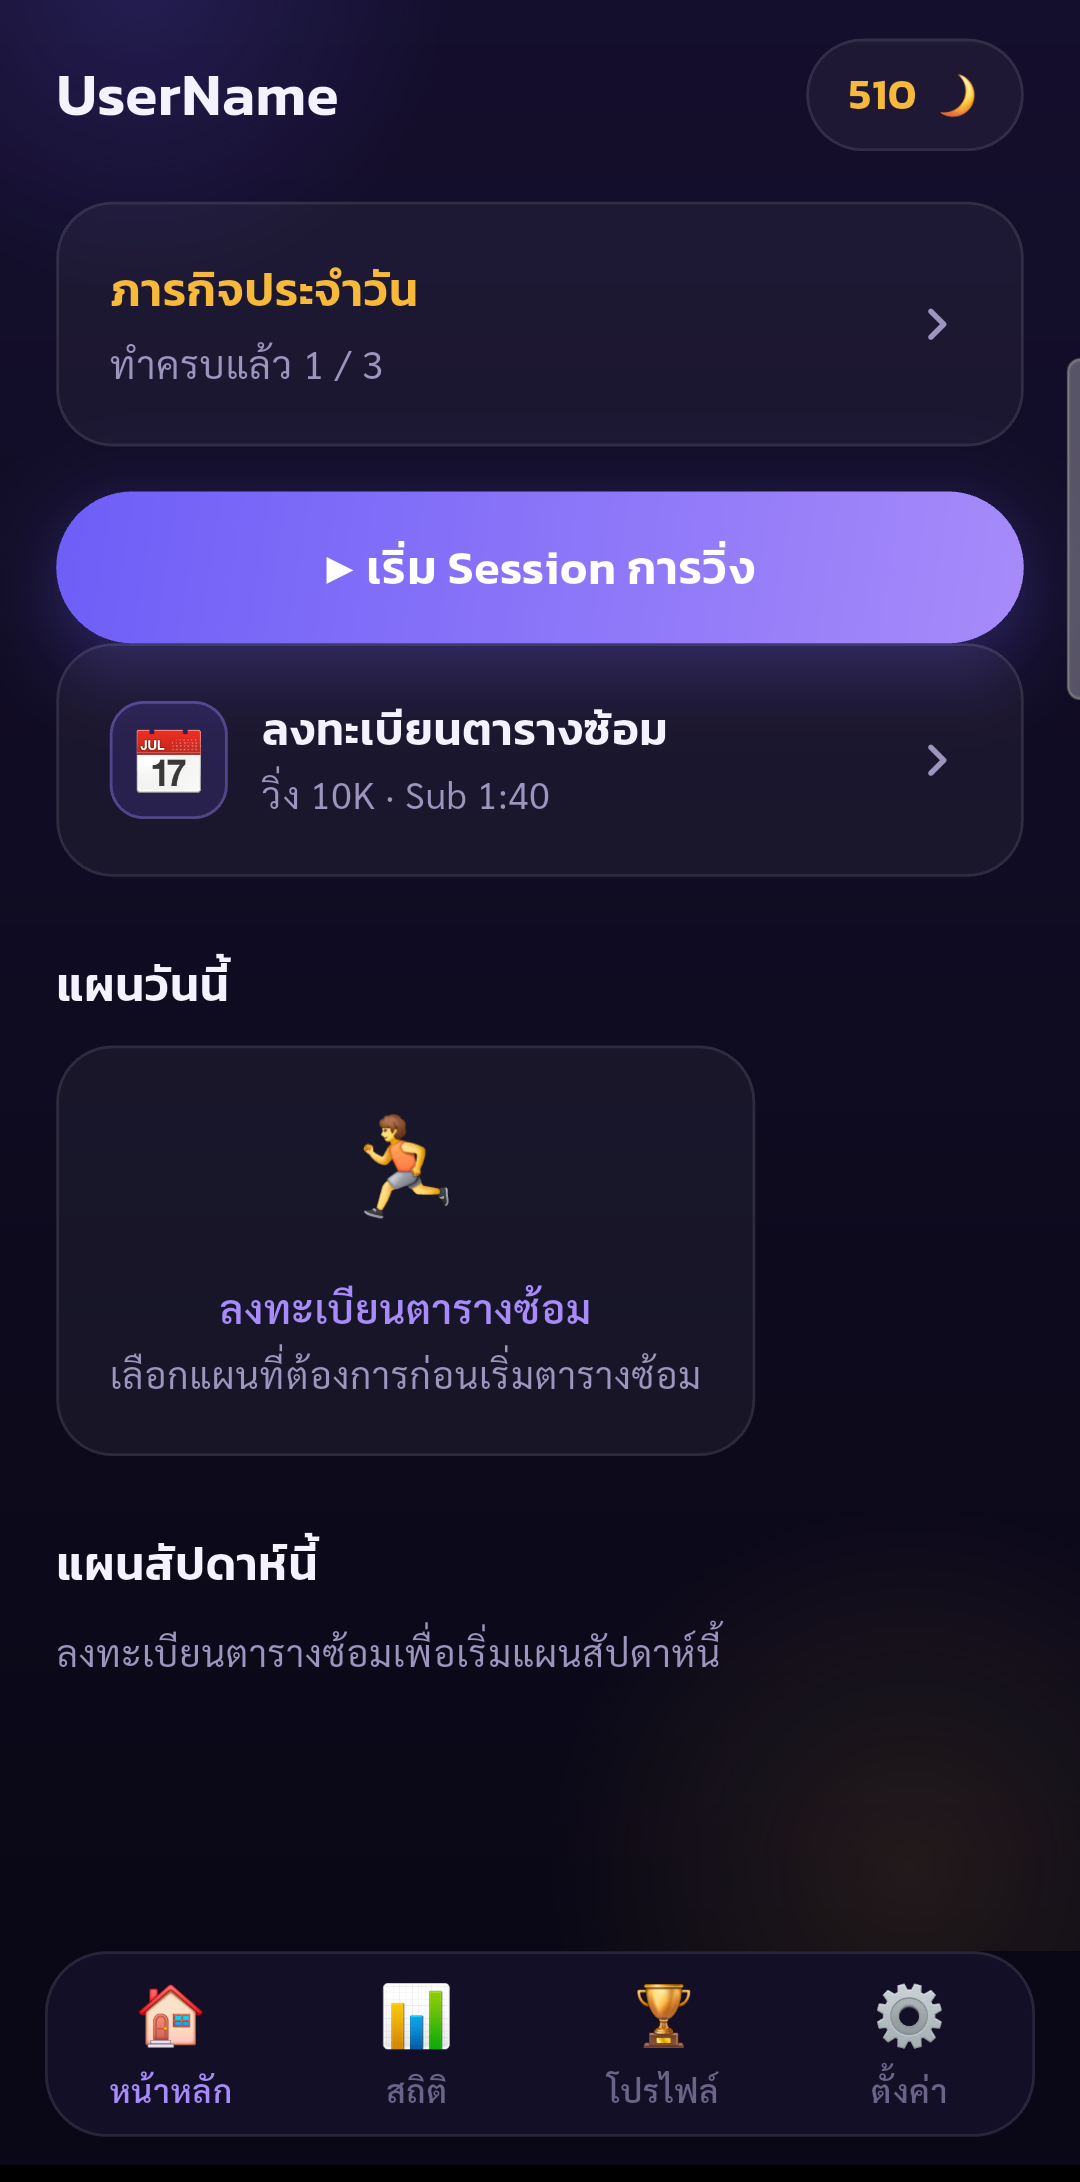
\includegraphics[width=\textwidth]{images/pegasus-home-training-required.png}\caption{หน้าหลักหลังการเช็กอิน}\end{subfigure}
\caption{หน้าหลักและการประเมินความพร้อมประจำวัน}\label{fig:app-home-wellness}\end{figure}

\begin{figure}[H]\centering
\begin{subfigure}[t]{0.31\textwidth}\centering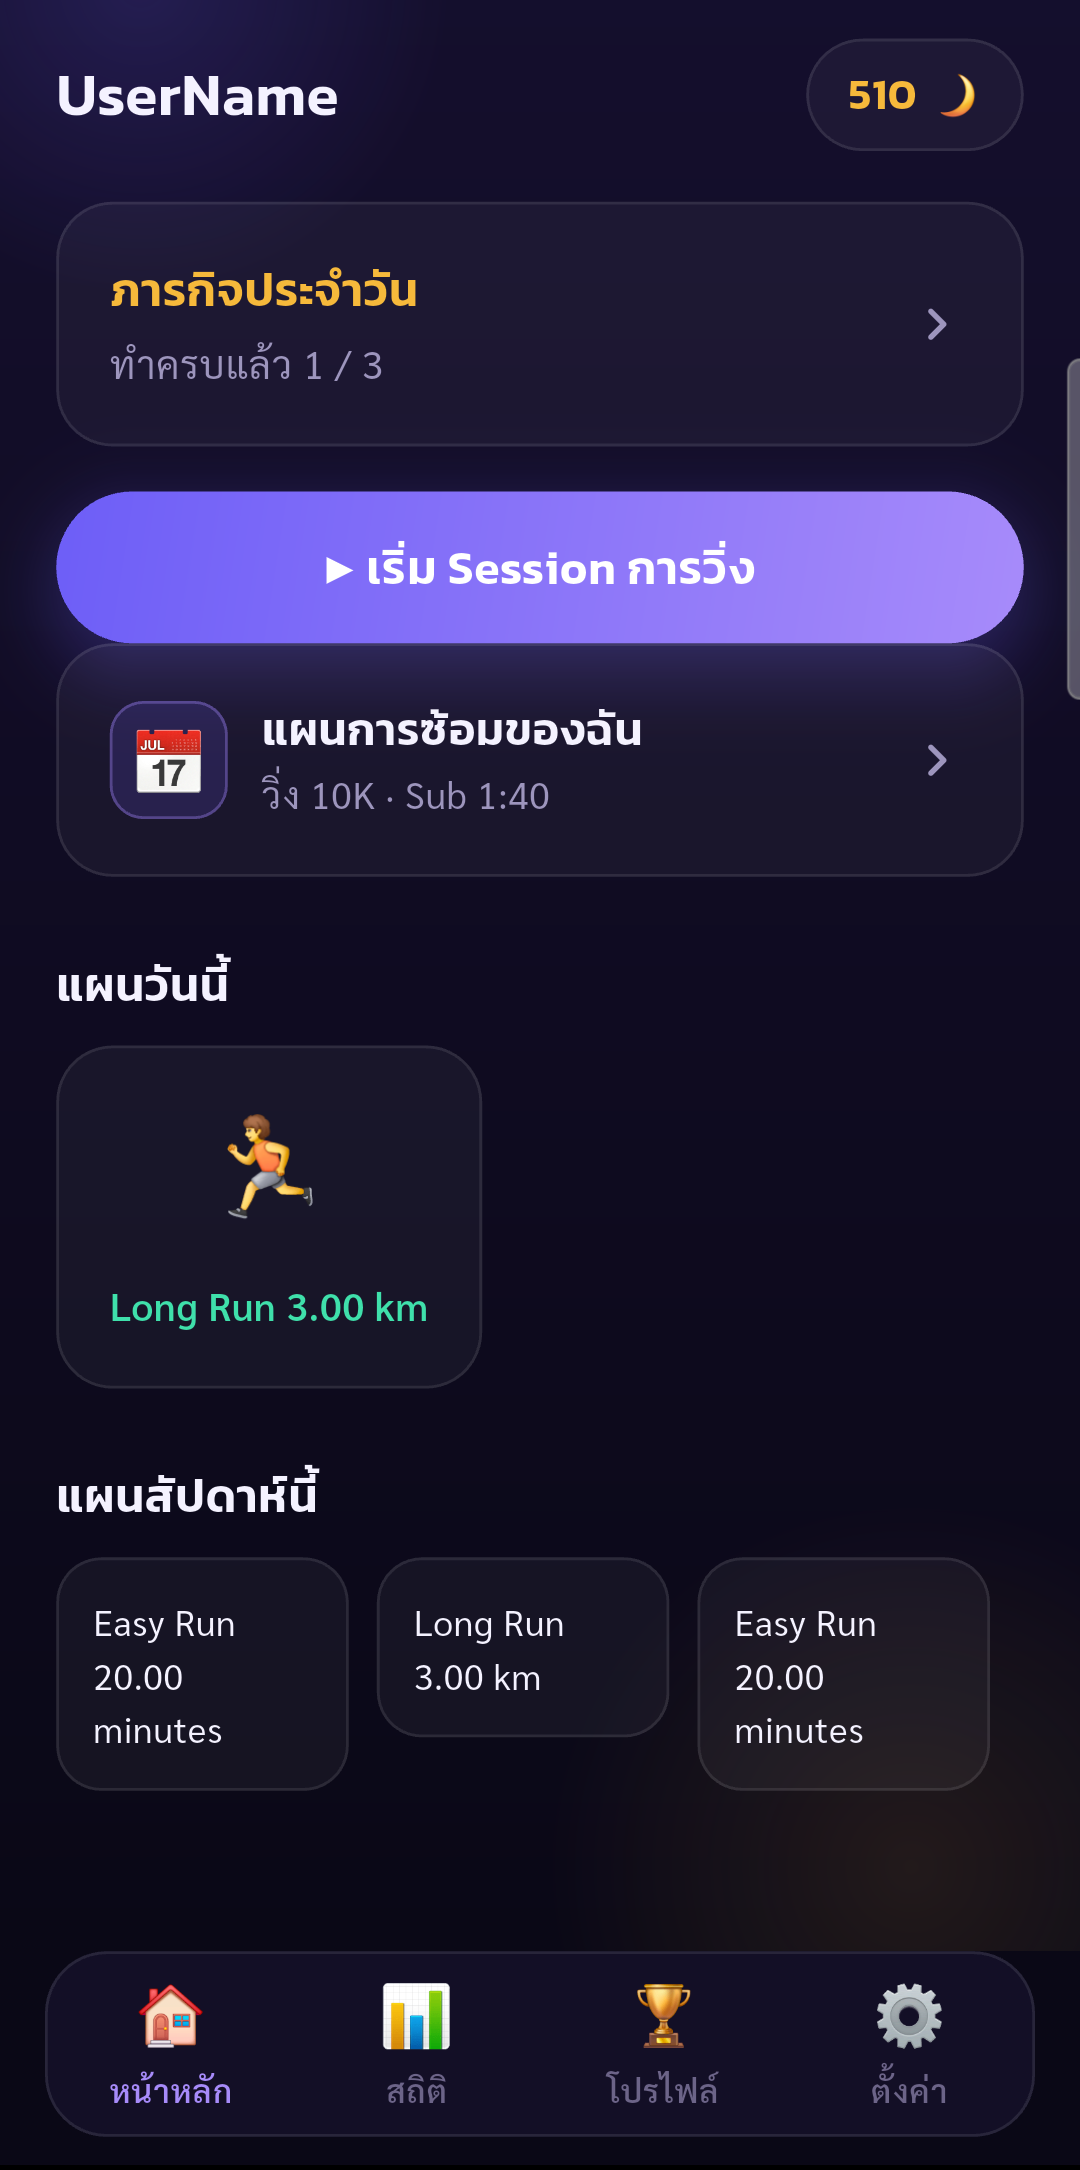
\includegraphics[width=\textwidth]{images/pegasus-home-training-scheduled.png}\caption{หน้าหลักพร้อมแผนฝึก}\end{subfigure}\hfill
\begin{subfigure}[t]{0.31\textwidth}\centering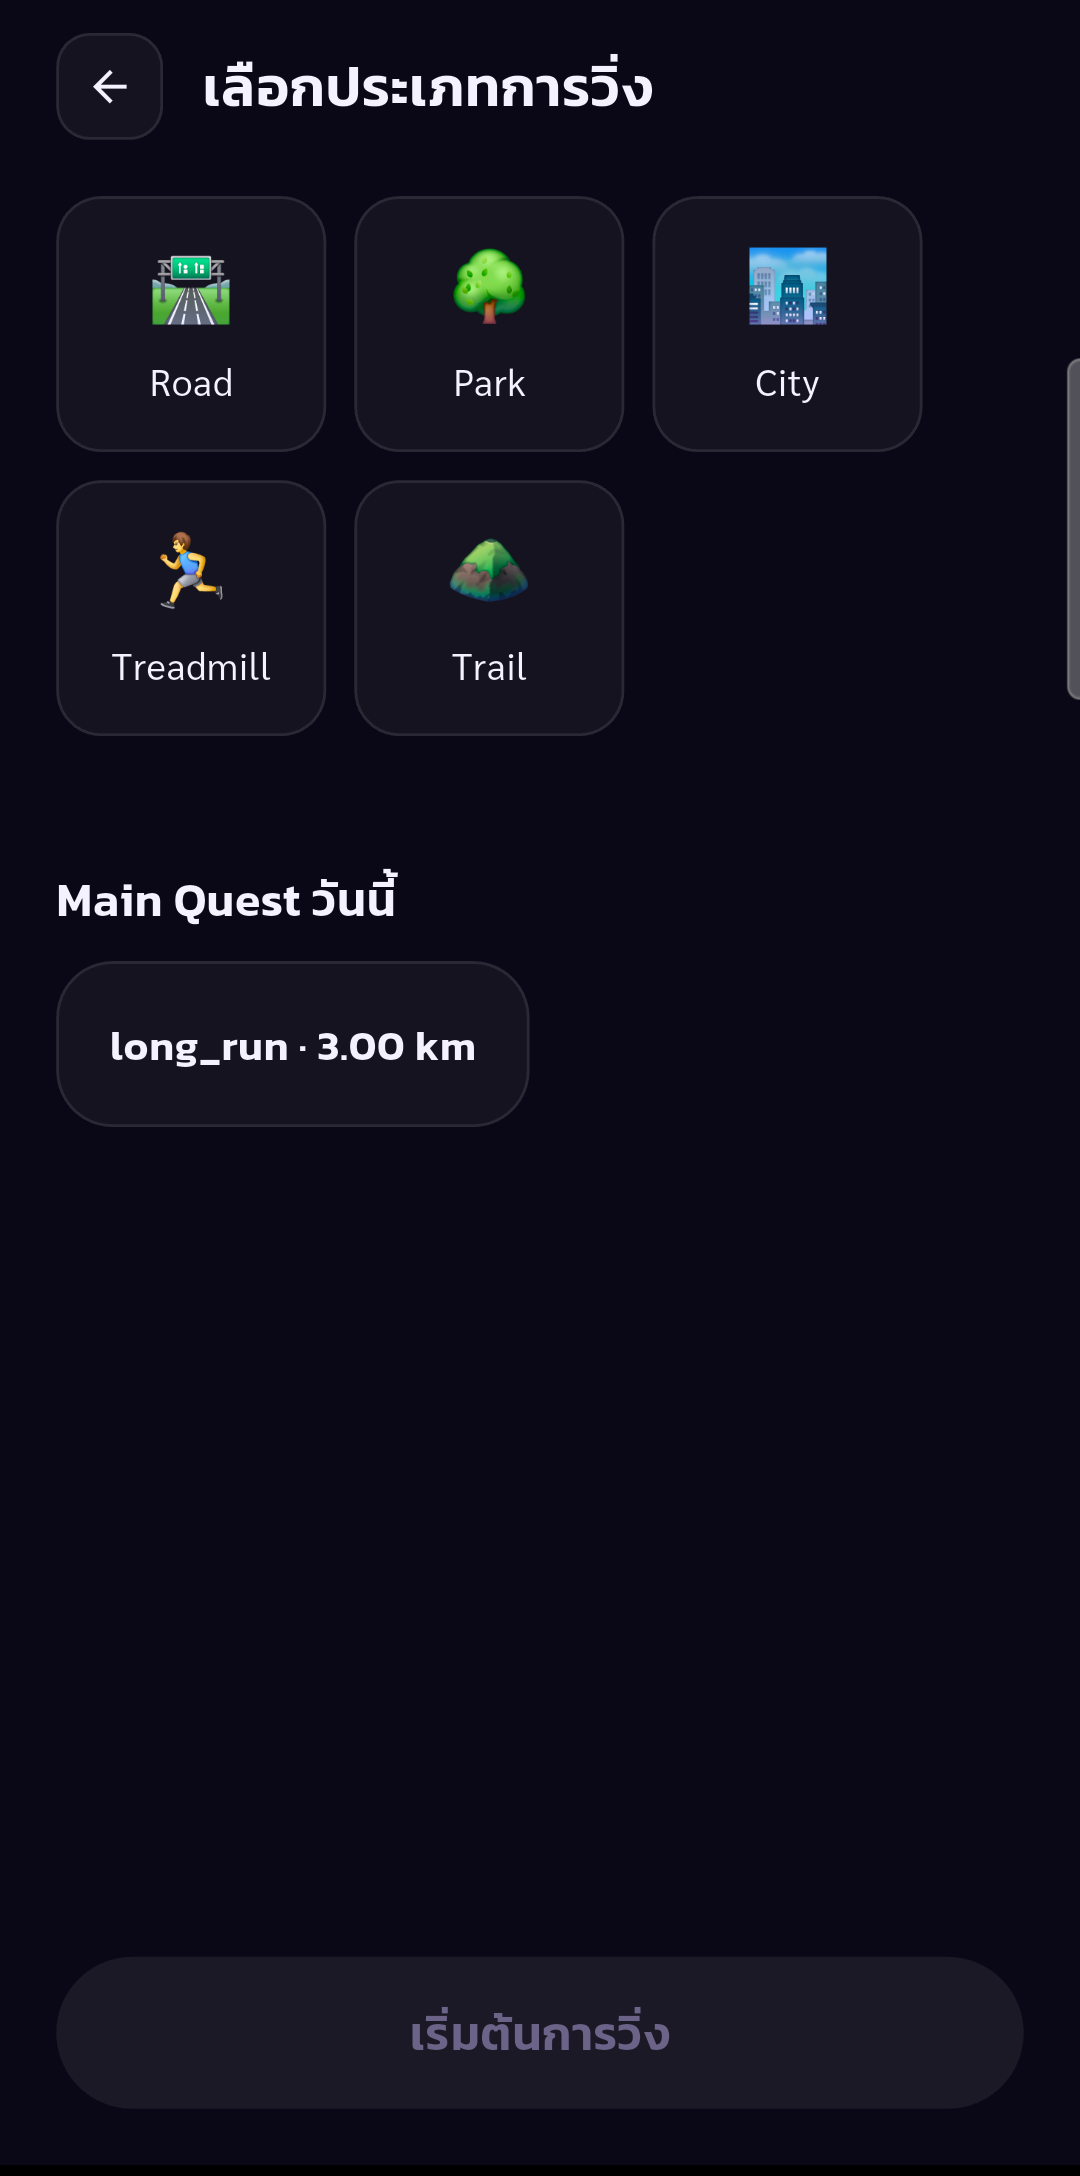
\includegraphics[width=\textwidth]{images/pegasus-run-session-type-selection.png}\caption{เลือกประเภทการวิ่ง}\end{subfigure}\hfill
\begin{subfigure}[t]{0.31\textwidth}\centering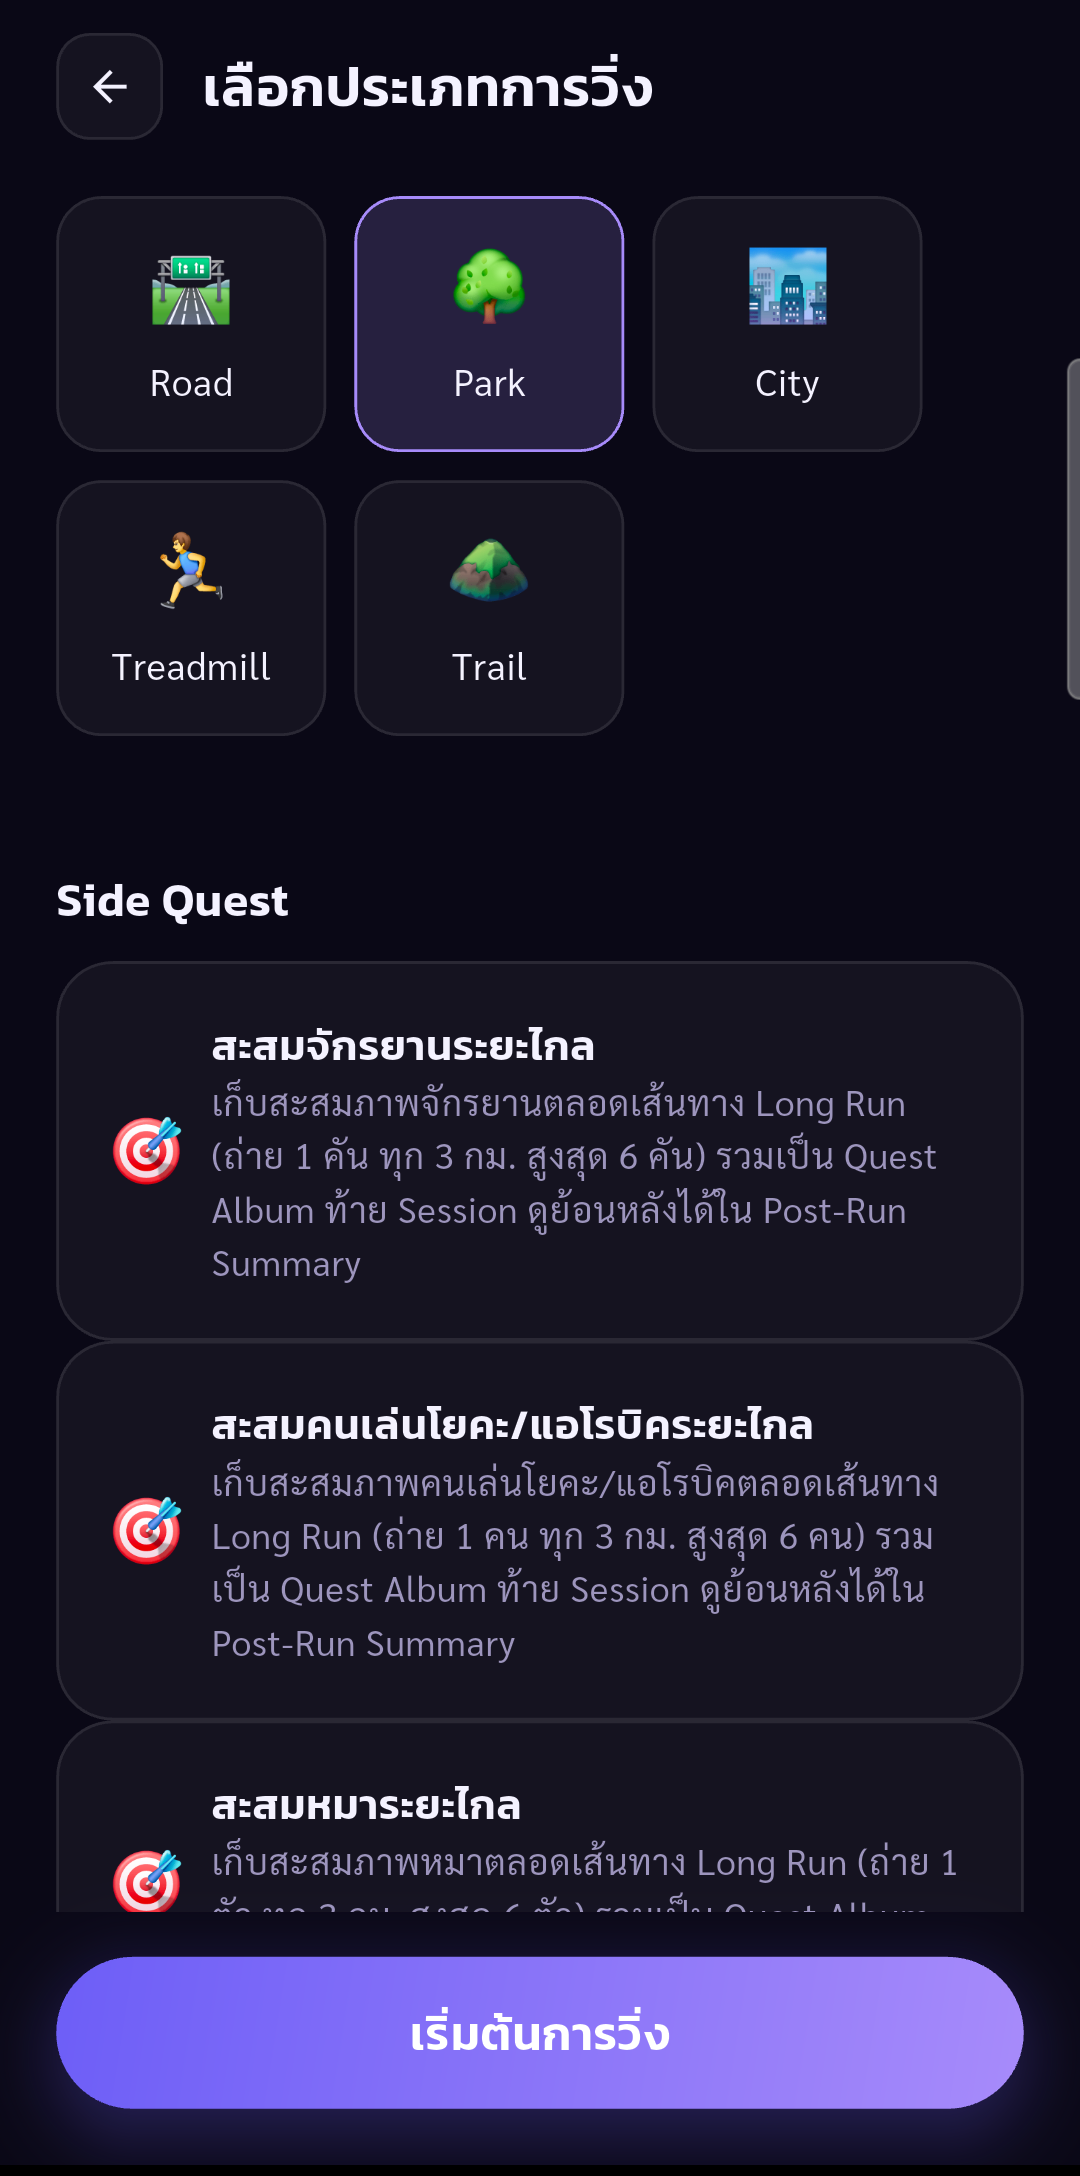
\includegraphics[width=\textwidth]{images/pegasus-run-session-quests.png}\caption{ภารกิจระหว่างการวิ่ง}\end{subfigure}
\caption{หน้าหลักและการเตรียมเริ่ม Session การวิ่ง}\label{fig:app-session-preparation}\end{figure}

\subsection{การวิ่งและผลลัพธ์หลังวิ่ง}

หน้าจอ Active Run Session แสดงเวลา ระยะทาง Pace ตำแหน่งบนแผนที่ และภารกิจที่กำลังดำเนินการ ผู้ใช้สามารถหยุดหรือจบการวิ่งได้ เมื่อจบการวิ่ง ระบบจะแสดงหน้าต่างยืนยันและหน้าสรุปผล เพื่อให้ผู้ใช้ประเมิน RPE ระดับความเครียด และความรู้สึกหลังวิ่ง

\begin{figure}[H]\centering
\begin{subfigure}[t]{0.31\textwidth}\centering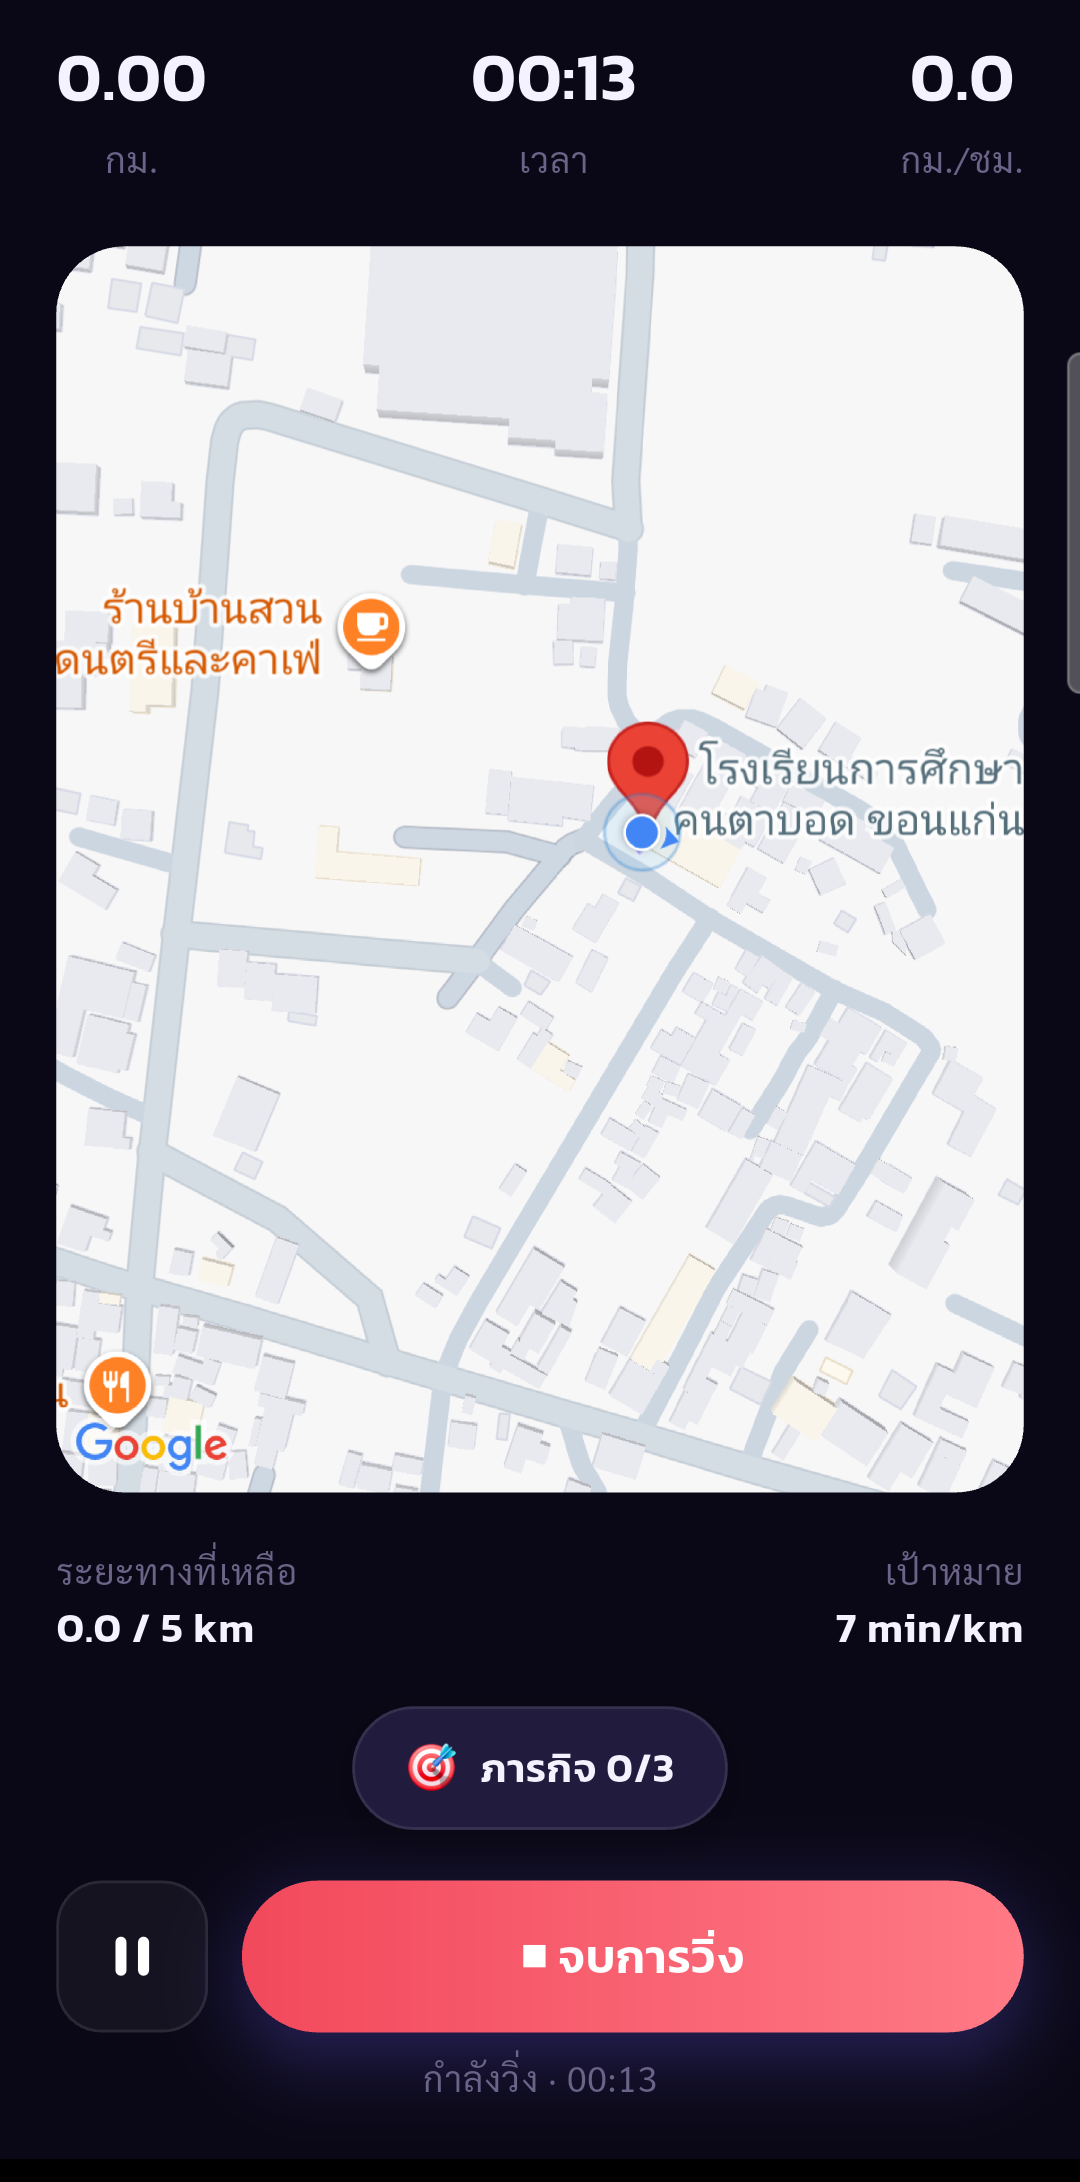
\includegraphics[width=\textwidth]{images/pegasus-active-run-session.png}\caption{กำลังวิ่ง}\end{subfigure}\hfill
\begin{subfigure}[t]{0.31\textwidth}\centering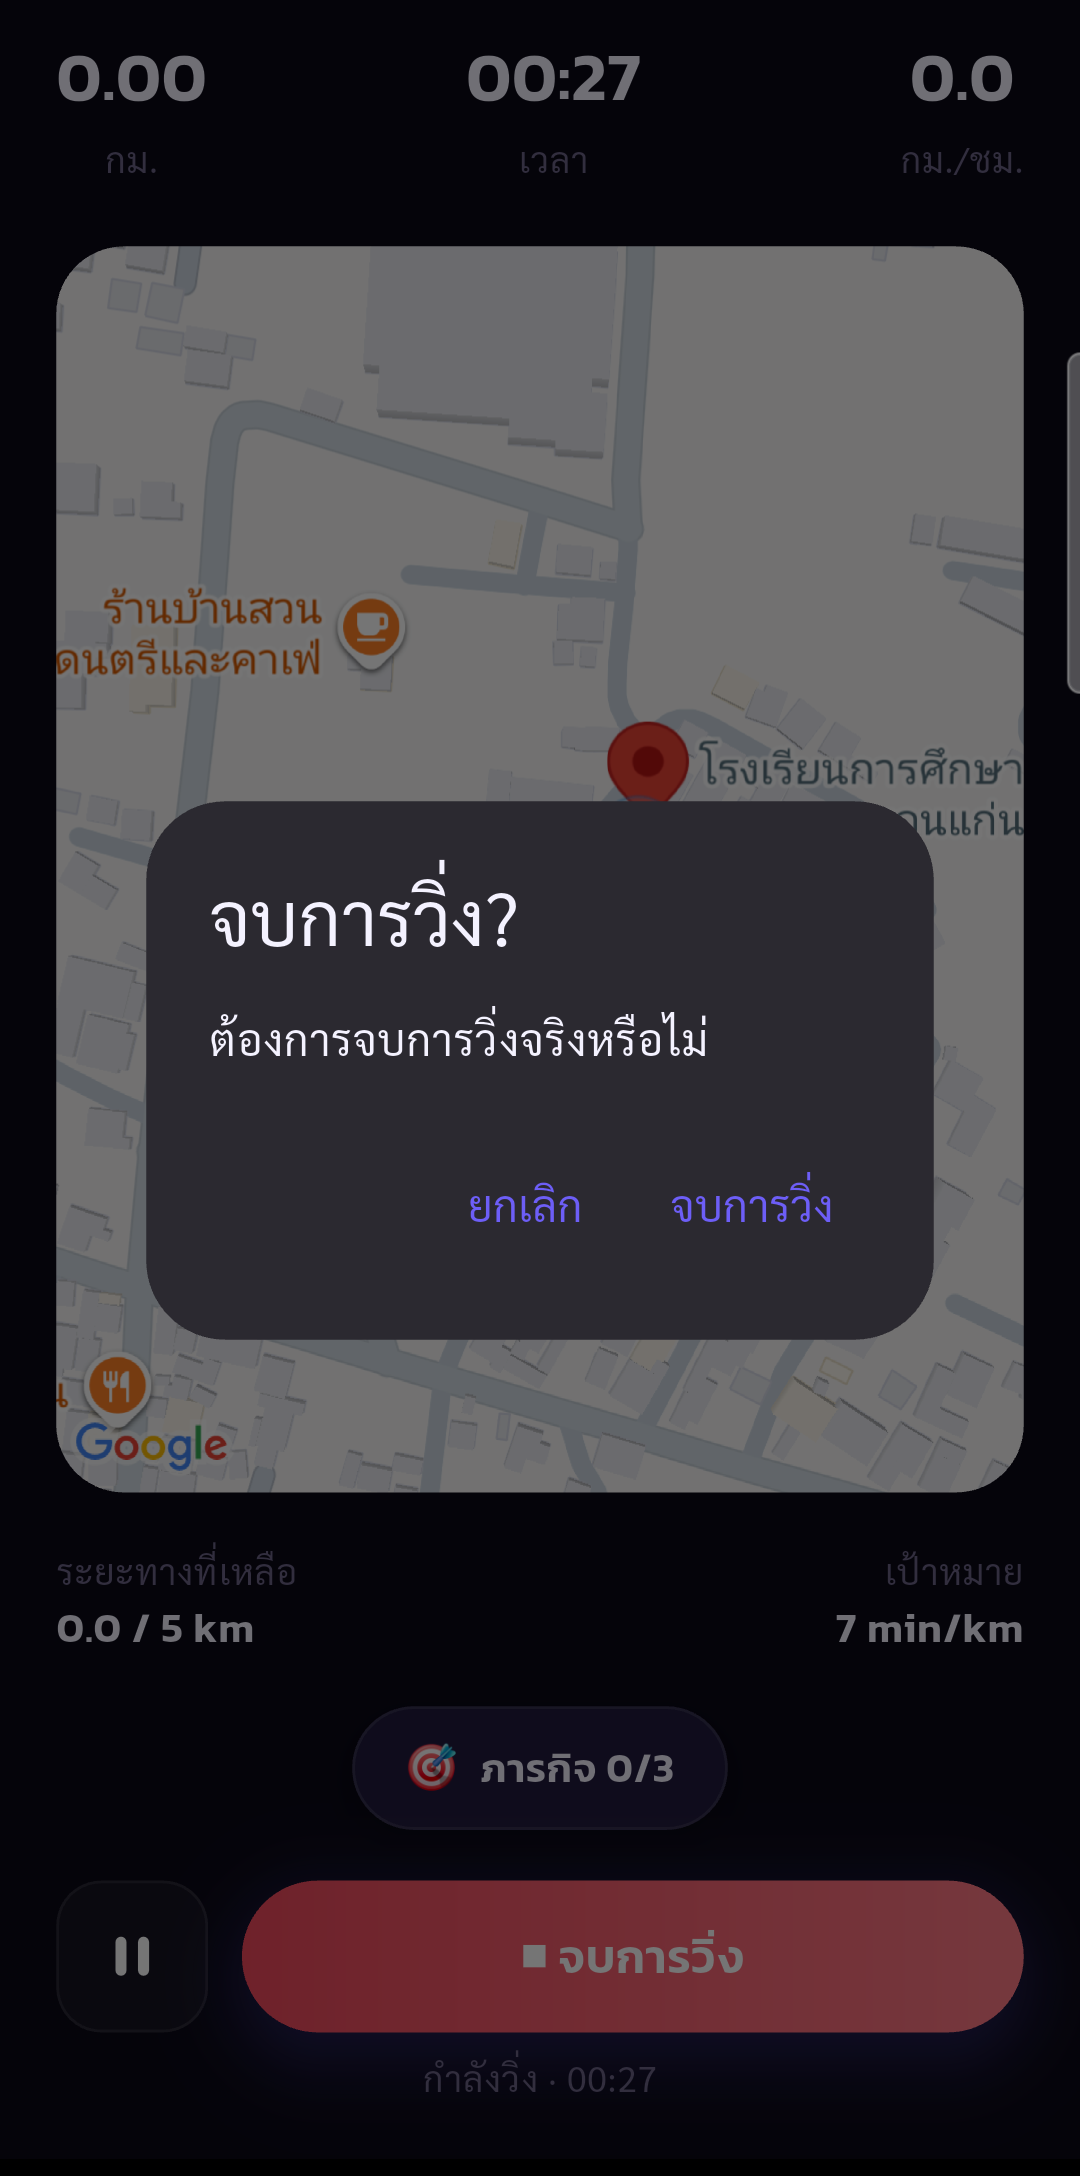
\includegraphics[width=\textwidth]{images/pegasus-end-run-confirmation.png}\caption{ยืนยันจบการวิ่ง}\end{subfigure}\hfill
\begin{subfigure}[t]{0.31\textwidth}\centering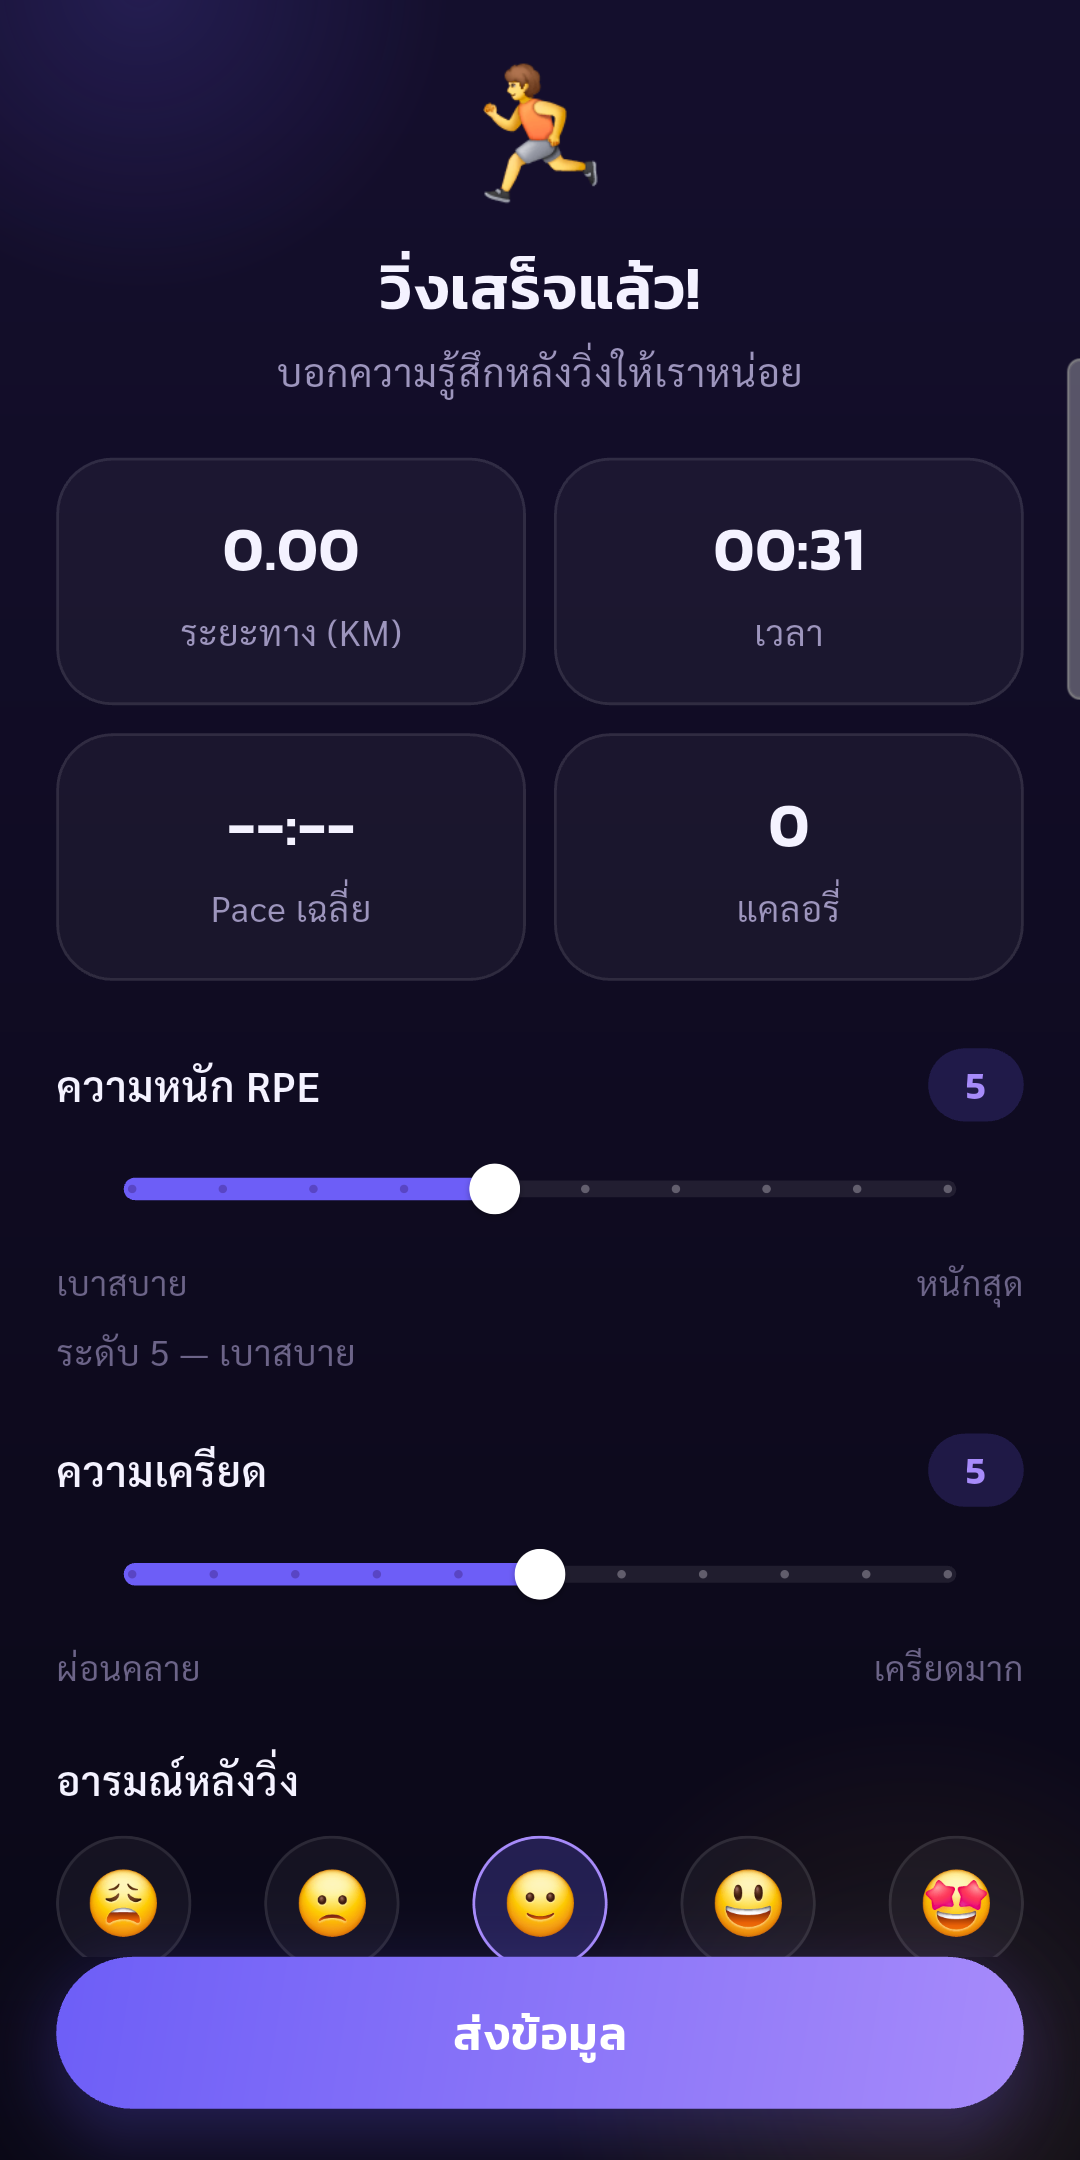
\includegraphics[width=\textwidth]{images/pegasus-post-run-feedback.png}\caption{สรุปผลและ Feedback}\end{subfigure}
\caption{หน้าจอการวิ่งและการประเมินหลังวิ่ง}\label{fig:app-running-result}\end{figure}

\subsection{ระบบรางวัลและ Gamification}

เมื่อผู้ใช้ทำกิจกรรมเสร็จ ระบบจะแสดงรางวัลเป็นเหรียญและคะแนนประสบการณ์ เพื่อสร้าง Feedback ทันทีและสนับสนุนให้ผู้ใช้กลับมาใช้งานอย่างต่อเนื่อง ผลการพัฒนาจึงครอบคลุมเส้นทางหลักตั้งแต่การสร้างบัญชี การเก็บข้อมูล การเลือกเป้าหมาย การเช็กอิน การวิ่ง ไปจนถึงการรับรางวัล

\begin{figure}[H]\centering

\includegraphics[width=0.31\textwidth]{images/pegasus-run-rewards.png}
\caption{หน้าจอแสดงรางวัลหลังการวิ่ง}\label{fig:app-rewards}\end{figure}

\section{ผลการออกแบบระบบ (System Design)}

จัดทำเอกสารการออกแบบระบบด้วย UML อย่างครบถ้วน เพื่อให้โครงสร้างระบบมีความชัดเจนและสามารถนำไปพัฒนาได้อย่างเป็นระบบ โดยแบ่ง Use Case Diagram ออกเป็น 12 แผนภาพย่อยตามกลุ่มฟังก์ชันการทำงาน ดังนี้

\subsection{Use Case Diagram}

\newcommand{\UseCaseFigure}[3]{%
\begin{figure}[H]\centering
\includegraphics[width=0.86\textwidth]{images/#1}
\caption{#2}\label{#3}
\end{figure}}

\subsubsection{Authentication System}
แสดงกระบวนการยืนยันตัวตนของนักวิ่ง ประกอบด้วยการสมัครสมาชิก การเข้าสู่ระบบด้วยบัญชีปกติหรือผ่าน Google และการออกจากระบบ โดยมี Actor หลักคือนักวิ่งและ Google
\UseCaseFigure{usecase-01.png}{Use Case Diagram Authentication System}{fig:usecase-authentication}

\subsubsection{กรอกข้อมูลพื้นฐาน}
แสดงกระบวนการตั้งค่าโปรไฟล์เริ่มต้นของนักวิ่ง ได้แก่ การกรอกข้อมูลส่วนตัว การเลือกอาการบาดเจ็บ การตั้งเป้าหมายการวิ่ง การกรอกประวัติการวิ่ง และการบันทึกโปรไฟล์ เพื่อให้ระบบนำข้อมูลไปปรับแผนฝึกได้อย่างเหมาะสม
\UseCaseFigure{usecase-02.png}{Use Case Diagram กรอกข้อมูลพื้นฐาน}{fig:usecase-basic-profile}

\subsubsection{Daily Wellness Check-in}
แสดงกระบวนการบันทึกสุขภาพประจำวันของนักวิ่ง ประกอบด้วยการบันทึกการนอนหลับ ความเหนื่อย ความเครียด และสภาพกล้ามเนื้อ รวมถึงการแก้ไขข้อมูลและรับ Coin +10 เมื่อบันทึกครบ
\UseCaseFigure{usecase-03.png}{Use Case Diagram Daily Wellness Check-in}{fig:usecase-wellness}

\subsubsection{Running Session}
แสดงกระบวนการบันทึกการวิ่งแบบเรียลไทม์ ตั้งแต่การเริ่ม Session การติดตาม GPS การทำภารกิจระหว่างวิ่ง การดูแผนที่วิ่ง การดูผลลัพธ์ การทำแบบทดสอบหลังวิ่ง และการรับรางวัล โดยเชื่อมต่อกับ Strava
\UseCaseFigure{usecase-04.png}{Use Case Diagram Running Session}{fig:usecase-running-session}

\subsubsection{แบบทดสอบหลังวิ่ง}
แสดงกระบวนการประเมินสภาพร่างกายหลังสิ้นสุด Session ประกอบด้วยการเลือกคะแนน RPE การเลือกสภาพร่างกาย ความรู้สึกหลังวิ่ง และการบันทึกแบบสอบถาม เพื่อนำข้อมูลไปปรับแผนฝึกในครั้งถัดไป
\UseCaseFigure{usecase-05.png}{Use Case Diagram แบบทดสอบหลังวิ่ง}{fig:usecase-post-run}

\subsubsection{Mission / Chapter}
แสดงกระบวนการทำภารกิจในระบบ Gamification ตั้งแต่การเลือก Chapter การทำ Mission การสิ้นสุด Mission การทำแบบทดสอบหลังวิ่ง และการรับรางวัล เพื่อสร้างแรงจูงใจในการออกกำลังกายอย่างต่อเนื่อง
\UseCaseFigure{usecase-06.png}{Use Case Diagram Mission / Chapter}{fig:usecase-mission}

\subsubsection{Club Create}
แสดงกระบวนการสร้างกลุ่มนักวิ่ง โดยนักวิ่งสามารถสร้าง Club ตั้งชื่อและตั้งค่า Club บันทึก และปิด Club ได้
\UseCaseFigure{usecase-07.png}{Use Case Diagram Club Create}{fig:usecase-club-create}

\subsubsection{Club Member}
แสดงกระบวนการเข้าร่วม Club โดยนักวิ่งสามารถค้นหา Club ส่งคำขอเข้าร่วม และออกจาก Club ได้ ในขณะที่ Club Leader สามารถตอบรับหรือปฏิเสธคำขอได้
\UseCaseFigure{usecase-08.png}{Use Case Diagram Club Member}{fig:usecase-club-member}

\subsubsection{Add Friends}
แสดงกระบวนการเพิ่มเพื่อนในระบบ โดยนักวิ่งสามารถค้นหาผู้ใช้ ส่งคำขอเป็นเพื่อน ตอบรับคำขอ ดูโปรไฟล์เพื่อน และลบเพื่อนได้ โดยมี Actor สองฝ่ายคือนักวิ่ง 1 และนักวิ่ง 2
\UseCaseFigure{usecase-09.png}{Use Case Diagram Add Friends}{fig:usecase-friends}

\subsubsection{Coin และ Item Shop}
แสดงกระบวนการใช้งานร้านค้าภายในระบบ นักวิ่งสามารถเข้าชมสินค้า เลือกหมวดหมู่ไอเทม ซื้อไอเทมด้วย Coin ดูไอเทมที่ซื้อแล้ว และนำไอเทมไปแต่งตัวได้
\UseCaseFigure{usecase-10.png}{Use Case Diagram Coin และ Item Shop}{fig:usecase-shop}

\subsubsection{Avatar 2.5D และ Avatar Dressing}
แสดงกระบวนการจัดการ Avatar ของนักวิ่งในรูปแบบ 2.5D ประกอบด้วยการดู Avatar การเลือกแต่งตัว การเลือกไอเทม การบันทึกการแต่งตัว และการกลับไปดูผลลัพธ์
\UseCaseFigure{usecase-11.png}{Use Case Diagram Avatar 2.5D และ Avatar Dressing}{fig:usecase-avatar}

\subsubsection{Leaderboard}
แสดงกระบวนการดูตารางอันดับของนักวิ่ง ประกอบด้วยการเข้าหน้า Leaderboard การเลือกกลุ่มจัดอันดับ การเลือกประเภทการจัดอันดับ และการดูโปรไฟล์ของผู้ใช้คนอื่น เพื่อสร้างแรงจูงใจในการแข่งขันและพัฒนาตนเอง
\UseCaseFigure{usecase-12.png}{Use Case Diagram Leaderboard}{fig:usecase-leaderboard}

\subsection{Use Case Description}

จัดทำ Use Case Description เพื่ออธิบายรายละเอียดของแต่ละ Use Case ในระบบ Pacegasus โดยแสดงในรูปแบบตาราง ประกอบด้วยชื่อ Use Case คำอธิบาย Actor เงื่อนไขก่อนเริ่ม เงื่อนไขหลังเสร็จ ขั้นตอนหลัก และกรณีผิดพลาด

\newcommand{\UseCaseTable}[7]{%
\begin{longtable}{|p{0.27\textwidth}|p{0.63\textwidth}|}
\caption{Use Case Description: #1}\\
\hline
\textbf{Use Case Name} & #1 \\\hline
\textbf{Description} & #2 \\\hline
\textbf{Actor} & #3 \\\hline
\textbf{Precondition} & #4 \\\hline
\textbf{Postcondition} & #5 \\\hline
\textbf{Main Success Scenario} & #6 \\\hline
\textbf{Exception} & #7 \\\hline
\end{longtable}
}

\UseCaseTable{สมัครสมาชิก}{ผู้ใช้ใหม่สร้างบัญชีโดยกรอกข้อมูลเพื่อเข้าใช้งานแอปพลิเคชัน}{นักวิ่ง}{ผู้ใช้ยังไม่มีบัญชีในระบบ}{ผู้ใช้มีบัญชีในระบบ}{1) ผู้ใช้เปิดแอปพลิเคชันและเลือกสมัครสมาชิก\newline 2) ระบบแสดงฟอร์มสมัครสมาชิก\newline 3) ผู้ใช้กรอกชื่อผู้ใช้ อีเมล รหัสผ่าน และยืนยันรหัสผ่าน\newline 4) ระบบตรวจสอบความถูกต้องของข้อมูล\newline 5) ระบบสร้างบัญชีและบันทึกลงฐานข้อมูล\newline 6) ระบบแจ้งว่าสมัครสมาชิกสำเร็จและนำไปยังหน้าเข้าสู่ระบบ}{E1: อีเมลซ้ำ แจ้งให้ใช้อีเมลอื่น\newline E2: รูปแบบอีเมลไม่ถูกต้อง\newline E3: รหัสผ่านไม่ตรงเงื่อนไข}

\UseCaseTable{เข้าสู่ระบบ}{ผู้ใช้ที่มีบัญชีอยู่แล้วยืนยันตัวตนด้วยอีเมลและรหัสผ่านเพื่อเข้าใช้งานระบบ}{นักวิ่ง}{ผู้ใช้มีบัญชีและยังไม่ได้เข้าสู่ระบบ}{ผู้ใช้เข้าสู่ระบบสำเร็จและอยู่ที่หน้าหลัก}{1) เปิดหน้าเข้าสู่ระบบ\newline 2) กรอกอีเมลและรหัสผ่าน\newline 3) ระบบตรวจสอบข้อมูลกับฐานข้อมูล\newline 4) ระบบนำผู้ใช้ไปยังหน้าหลัก}{อีเมลหรือรหัสผ่านไม่ถูกต้อง ระบบแจ้งเตือนโดยไม่ระบุว่าผิดข้อใด}

\UseCaseTable{เข้าสู่ระบบด้วย Google}{ผู้ใช้ยืนยันตัวตนผ่าน Google OAuth แทนการใช้รหัสผ่านของระบบ}{นักวิ่ง, Google}{ผู้ใช้มีบัญชี Google และยังไม่ได้เข้าสู่ระบบ}{ผู้ใช้เข้าสู่ระบบสำเร็จผ่าน Google OAuth และอยู่ที่หน้าหลัก}{1) กดเข้าสู่ระบบด้วย Google\newline 2) ระบบเปิดหน้าต่าง Google OAuth\newline 3) เลือกบัญชีและอนุมัติสิทธิ์\newline 4) Google ส่งโทเคนกลับมา\newline 5) ระบบสร้างบัญชีโดยอัตโนมัติ\newline 6) ระบบนำไปยังหน้าหลัก}{E1: ผู้ใช้ยกเลิก OAuth ระบบกลับสู่หน้าเข้าสู่ระบบ\newline E2: Google ปฏิเสธคำขอ ระบบแจ้งข้อผิดพลาด}

\UseCaseTable{ออกจากระบบ}{ผู้ใช้ออกจากแอปพลิเคชันอย่างปลอดภัย}{นักวิ่ง}{ผู้ใช้เข้าสู่ระบบอยู่}{Session ถูกลบออกและผู้ใช้กลับไปหน้าเข้าสู่ระบบ}{1) กดออกจากระบบ\newline 2) ระบบแสดงหน้าต่างยืนยัน\newline 3) ผู้ใช้กดยืนยัน\newline 4) ระบบนำผู้ใช้ออกจากบัญชีและกลับไปหน้า Login}{ผู้ใช้กดยกเลิก ระบบปิดหน้าต่างและยังอยู่ในแอป}

\UseCaseTable{กรอกข้อมูลพื้นฐาน}{ผู้ใช้ป้อนข้อมูลส่วนตัวเบื้องต้น เช่น ชื่อ อายุ น้ำหนัก ส่วนสูง และเพศ เพื่อให้ระบบปรับแผนการวิ่ง}{นักวิ่ง}{เข้าสู่ระบบแล้วและยังไม่ได้กรอกข้อมูลพื้นฐาน}{ข้อมูลพื้นฐานถูกบันทึกและเข้าสู่ขั้นตอนถัดไป}{1) ระบบแสดงฟอร์มข้อมูลพื้นฐาน\newline 2) ผู้ใช้กรอกข้อมูล\newline 3) ระบบตรวจสอบความครบถ้วนและความถูกต้อง\newline 4) ระบบบันทึกข้อมูลและไปขั้นตอนถัดไป}{ข้อมูลไม่ครบหรือไม่ถูกต้อง ระบบแจ้งเตือนใต้ช่องที่ผิดพลาด}

\UseCaseTable{เลือกอาการบาดเจ็บและโรคประจำตัว}{ผู้ใช้ระบุอาการบาดเจ็บและโรคประจำตัว เพื่อให้ระบบหลีกเลี่ยงแผนฝึกที่อาจก่อความเสี่ยง}{นักวิ่ง}{กรอกข้อมูลพื้นฐานเสร็จแล้ว}{ข้อมูลถูกบันทึกเพื่อใช้ปรับแผนฝึก}{1) ระบบแสดงรายการอาการและโรค\newline 2) ผู้ใช้เลือกได้หลายรายการหรือเลือกไม่มี\newline 3) ระบบบันทึกข้อมูลและดำเนินการต่อ}{ไม่มีรายการผิดพลาดที่ระบุไว้ในเอกสารต้นฉบับ}

\UseCaseTable{กรอกประวัติการวิ่ง}{ผู้ใช้บันทึกประสบการณ์การวิ่งในอดีต เพื่อให้ระบบประเมินระดับความฟิตเบื้องต้น}{นักวิ่ง}{กรอกข้อมูลพื้นฐานเสร็จแล้ว}{ประวัติการวิ่งถูกบันทึกเพื่อนำไปประเมินระดับความฟิต}{1) ระบบแสดงฟอร์มประวัติการวิ่ง\newline 2) ผู้ใช้กรอกระยะทางเฉลี่ยต่อสัปดาห์ ความถี่ และระดับประสบการณ์\newline 3) ระบบบันทึกข้อมูลและดำเนินการต่อ}{กรอกข้อมูลไม่ครบ ระบบแจ้งให้กรอกใหม่}

\UseCaseTable{ตั้งเป้าหมายการวิ่ง}{ผู้ใช้กำหนดเป้าหมายการวิ่งระยะยาว เช่น ลดน้ำหนักหรือเตรียมพร้อมสำหรับงานวิ่ง}{นักวิ่ง}{กรอกประวัติการวิ่งเสร็จแล้ว}{เป้าหมายถูกบันทึกเพื่อนำไปกำหนดแผนฝึก}{1) ระบบแสดงรายการเป้าหมาย\newline 2) ผู้ใช้เลือกเป้าหมายและกำหนดระยะเวลา\newline 3) ระบบบันทึกเป้าหมายและดำเนินการต่อ}{ไม่ได้เลือกเป้าหมาย ระบบแจ้งให้เลือกอย่างน้อย 1 รายการ}

\UseCaseTable{บันทึกโปรไฟล์}{ระบบรวบรวมข้อมูลทุกส่วนที่ผู้ใช้กรอกและบันทึกเป็นโปรไฟล์ที่สมบูรณ์}{นักวิ่ง}{กรอกข้อมูลครบทุกส่วนแล้ว}{โปรไฟล์ถูกบันทึกครบถ้วนและผู้ใช้เข้าสู่หน้าหลัก}{1) กดบันทึกโปรไฟล์\newline 2) ระบบรวบรวมและตรวจสอบข้อมูล\newline 3) ระบบบันทึกโปรไฟล์ลงฐานข้อมูล\newline 4) ระบบแสดงข้อความยืนยันและนำไปหน้าหลัก}{เกิดข้อผิดพลาดในการบันทึก ระบบแจ้งเตือนและให้ลองใหม่}

\UseCaseTable{Daily Wellness Check-in}{ผู้ใช้บันทึกสภาพร่างกายและจิตใจประจำวัน ได้แก่ การนอนหลับ ความเหนื่อย ความเครียด และสภาพกล้ามเนื้อ เพื่อติดตามความพร้อมในการวิ่ง}{นักวิ่ง}{เข้าสู่ระบบแล้วและยังไม่ได้เช็กอินวันนี้}{ข้อมูล Daily Wellness ถูกบันทึกและผู้ใช้ได้รับเหรียญรางวัล}{1) เปิดเมนู Daily Wellness Check-in\newline 2) ระบบแสดงหัวข้อ 4 หมวด\newline 3) บันทึกชั่วโมงและคุณภาพการนอน\newline 4) เลือกระดับความเหนื่อย 1--10\newline 5) เลือกระดับความเครียด 1--10\newline 6) เลือกสภาพกล้ามเนื้อ\newline 7) กดบันทึก\newline 8) ระบบบันทึกข้อมูลและให้รางวัล}{ข้อมูลการนอนไม่ถูกต้อง เช่น เกิน 24 ชั่วโมง ระบบแจ้งเตือน}

\UseCaseTable{เริ่มเซสชันการวิ่ง}{ผู้ใช้เริ่มบันทึกการวิ่งและระบบเริ่มติดตาม GPS}{นักวิ่ง}{เข้าสู่ระบบ เปิด GPS และมีการเชื่อมต่ออินเทอร์เน็ต}{เซสชันการวิ่งเริ่มต้นและระบบกำลังติดตาม GPS}{1) กดเริ่มวิ่ง\newline 2) ระบบตรวจสอบสัญญาณ GPS\newline 3) ระบบติดตามตำแหน่งและบันทึกแบบ Real-time\newline 4) ระบบแสดงระยะทาง เวลา ความเร็ว และแผนที่}{ไม่มีสัญญาณ GPS ระบบแจ้งเตือนและให้เปิด GPS ก่อน}

\UseCaseTable{ทำภารกิจระหว่างวิ่ง}{ผู้ใช้เลือกและทำภารกิจระหว่างเซสชันการวิ่งเพื่อรับรางวัลพิเศษ}{นักวิ่ง}{เซสชันการวิ่งกำลังดำเนินอยู่}{ภารกิจถูกบันทึกว่าสำเร็จและได้รับรางวัล}{1) เลือกภารกิจระหว่างวิ่ง\newline 2) ระบบแสดงรายละเอียดและเงื่อนไข\newline 3) ผู้ใช้ทำภารกิจสำเร็จ\newline 4) ระบบบันทึกผลและให้รางวัล}{ผู้ใช้ยกเลิกภารกิจ ระบบบันทึกว่าไม่สำเร็จ}

\UseCaseTable{กดจบเซสชันการวิ่ง}{ผู้ใช้จบการวิ่ง ระบบหยุดติดตามและบันทึกข้อมูลทั้งหมด}{นักวิ่ง}{เซสชันการวิ่งกำลังดำเนินอยู่}{เซสชันสิ้นสุด ข้อมูลถูกบันทึก และผู้ใช้อยู่หน้าผลลัพธ์}{1) กดจบการวิ่ง\newline 2) ระบบหยุดติดตาม GPS\newline 3) ระบบบันทึกข้อมูลการวิ่งลงฐานข้อมูล\newline 4) ระบบแสดงผลลัพธ์การวิ่ง}{ข้อมูล GPS สูญหายบางส่วน ระบบบันทึกข้อมูลที่มีอยู่}

\UseCaseTable{ดูผลลัพธ์การวิ่ง}{ระบบสรุปและแสดงสถิติการวิ่งหลังจบ Session พร้อมตัวเลือกแชร์}{นักวิ่ง}{เซสชันการวิ่งสิ้นสุดแล้ว}{ผู้ใช้รับทราบสถิติครบถ้วนและสามารถแชร์ผลลัพธ์}{1) ระบบแสดงระยะทาง เวลา ความเร็วเฉลี่ย และแคลอรี่\newline 2) ผู้ใช้ดูข้อมูลรายละเอียด}{ไม่มีกรณีผิดพลาดที่ระบุไว้ในเอกสารต้นฉบับ}

\UseCaseTable{ทำแบบทดสอบหลังวิ่ง}{ผู้ใช้ตอบแบบสอบถามสั้น ๆ เกี่ยวกับความรู้สึกและสภาพร่างกายหลังวิ่ง}{นักวิ่ง}{เซสชันการวิ่งสิ้นสุดแล้ว}{ข้อมูลถูกบันทึกเพื่อวิเคราะห์และปรับแผน พร้อมรับรางวัล}{1) ระบบแสดงแบบทดสอบ\newline 2) เลือกคะแนน RPE 1--10\newline 3) เลือกสภาพร่างกาย\newline 4) เลือกความรู้สึกหลังวิ่ง\newline 5) กดบันทึกแบบสอบถาม\newline 6) ได้รับรางวัล}{ทำแบบทดสอบไม่ครบ ระบบแจ้งเตือนให้ทำให้ครบ}

\UseCaseTable{เลือกบท}{ผู้ใช้เลือกบทที่ต้องการเพื่อดูภารกิจและเนื้อหาภายใน}{นักวิ่ง}{เข้าสู่ระบบและอยู่ในส่วนภารกิจ/บท}{เห็นรายการภารกิจทั้งหมดภายในบทที่เลือก}{1) ระบบแสดงบททั้งหมดพร้อมสถานะ\newline 2) ผู้ใช้เลือกบท\newline 3) ระบบแสดงภารกิจทั้งหมดใน Chapter}{บทถูกล็อก ระบบแสดงเงื่อนไขการปลดล็อก}

\UseCaseTable{ทำภารกิจ}{ผู้ใช้เริ่มทำภารกิจที่กำหนดไว้ในบทเพื่อรับรางวัลและความก้าวหน้า}{นักวิ่ง}{เลือกบทแล้วและภารกิจยังไม่สำเร็จ}{ภารกิจเริ่มต้นและระบบติดตามความก้าวหน้า}{1) เลือกภารกิจ\newline 2) ระบบแสดงรายละเอียดและเงื่อนไข\newline 3) กดเริ่มภารกิจพร้อมเซสชันการวิ่ง\newline 4) ระบบบันทึกความก้าวหน้า}{ระดับผู้ใช้ไม่เพียงพอ ระบบแจ้งเงื่อนไขที่ต้องปลดล็อก}

\UseCaseTable{กดจบภารกิจ}{ผู้ใช้จบภารกิจ ระบบประมวลผลและให้รางวัล}{นักวิ่ง}{ภารกิจกำลังดำเนินอยู่}{ภารกิจสิ้นสุด ผลถูกบันทึก และได้รับรางวัลหากบรรลุเงื่อนไข}{1) กดจบภารกิจ\newline 2) ระบบตรวจสอบเงื่อนไข\newline 3) ระบบบันทึกผลและแสดงสรุป\newline 4) ระบบนำไปทำแบบทดสอบหลังวิ่ง\newline 5) ระบบให้รางวัลเมื่อสำเร็จ}{ไม่มีกรณีผิดพลาดที่ระบุไว้ในเอกสารต้นฉบับ}

\section{สรุปผลการพัฒนา}

ผลการดำเนินงานในบทนี้แสดงให้เห็นว่า Pacegasus สามารถพัฒนาเป็นแอปพลิเคชันต้นแบบที่รองรับเส้นทางการใช้งานหลักได้ครบถ้วน ตั้งแต่การเข้าสู่ระบบและสมัครสมาชิก การยืนยัน OTP การกรอกข้อมูลพื้นฐานและข้อมูลสุขภาพ การกำหนดเป้าหมาย การเลือกแผนการฝึก การประเมินความพร้อมประจำวัน การเริ่ม Session การวิ่ง การประเมินหลังวิ่ง และการรับรางวัล

นอกจากนี้ โครงสร้างระบบยังเตรียมรองรับการเชื่อมต่อ Strava API, การประเมินภาระการฝึกด้วย Session-RPE และ ACWR รวมถึงการต่อยอดระบบสังคมและ Machine Learning ในระยะถัดไป 